%%%%%%%%%%%%%%%%%%%%%%%%%%%%%%%%%%%%%%%%%
%
% Ciência e Natura LaTeX Template
% Version 1.0 (19/01/2017)
%
%%%%%%%%%%%%%%%%%%%%%%%%%%%%%%%%%%%%%%%%%

%----------------------------------------------------------------------------------------
%	DOCUMENT CONFIGURATIONS (not for authors)
%----------------------------------------------------------------------------------------
\documentclass[twoside,a4paper,10pt]{article}

%\usepackage[brazilian]{babel}
\usepackage[english,brazil]{babel}

\usepackage[utf8]{inputenc}% acentuação (se esse não funcionar use a linha abaixo)
%\usepackage[latin1]{inputenc} %acentuação (windows)
\usepackage[T1]{fontenc} % Use 8-bit encoding that has 256 glyphs

%----------------------------------------------------------------------------------------
%	PAPER INFORMATION 
%----------------------------------------------------------------------------------------
\newcommand{\shorttitle}{Felipe Barbosa}


%----------------------------------------------------------------------------------------
%	TEMPLATE CONFIGURATIONS (not for authors)
%----------------------------------------------------------------------------------------
\usepackage{authblk} % Package to Prepare Author and Affiliation Blocks
\usepackage{lipsum} % Package to generate dummy text throughout this template
\usepackage{times}
\usepackage{microtype} % Slightly tweak font spacing for aesthetics
\usepackage[hmarginratio=1:1,top=33mm,columnsep=20pt,text={18cm,24.3cm}]{geometry} % Document margins
\usepackage{booktabs} % Horizontal rules in tables
\usepackage{abstract} % Allows abstract customization
\renewcommand{\abstractnamefont}{\normalfont\bfseries} % Set the "Abstract" text to bold
\renewcommand{\abstracttextfont}{\normalfont\small\itshape} % Set the abstract itself to small italic text
\newcommand{\titleeng}{\vspace{4mm}\fontsize{14pt}{14pt}
\selectfont}
\newcommand{\titlept}{\textbf} % título em português
\usepackage{titlesec} % Allows customization of titles
\usepackage{fancyhdr} % Headers and footers
\pagestyle{fancy} % All pages have headers and footers
\fancyfoot{} % Blank out the default footer
\fancyhead[EL]{Ciência e Natura} % 
\fancyhead[ER]{\thepage} % Custom header text
\fancyhead[OR]{Autores: \shorttitle} % Custom header text
\fancyhead[OL]{\thepage} % Custom header text

\renewcommand\Authand{ e } % separação do nome dos autores (portugues)
\renewcommand\Authands{ e } % separação do nome dos autores (portugues)

%\renewcommand\Authand{ and } % separação do nome dos autores (ingles)
%\renewcommand\Authands{ and } % separação do nome dos autores (ingles)



%----------------------------------------------------------------------------------------
%	YOUR PACKAGES
%----------------------------------------------------------------------------------------
\usepackage{amssymb,amsmath,amsthm,amsfonts} % math
\usepackage{natbib} % for \citep 
\usepackage{graphicx,rotating} 
\usepackage{enumerate}
\usepackage{graphics}
\usepackage[dvips]{epsfig}
\usepackage{multirow}
\usepackage{nonfloat}
\usepackage{multicol} % Used for the two-column layout of the document
\usepackage{url} % hiperlink
\usepackage{hyperref} % For hyperlinks in the PDF
\usepackage{subfigure} % subfigures
\usepackage{bm}
\usepackage{color}
\usepackage{icomma} % ajusta vírgula como separador decimal (textos em portugues)
%\usepackage{refcheck} % checar referencias cruzadas

\allowdisplaybreaks[4] % para evitar espaços entre fórmulas


%----------------------------------------------------------------------------------------
%	YOUR NEW COMMANDS
%----------------------------------------------------------------------------------------
\newcommand{\Z}{\mathbb Z} % conjunto dos números inteiros
\newcommand{\R}{\mathbb R} % conjunto dos números reais
\newtheorem{mydef}{Definicão}[section]


%----------------------------------------------------------------------------------------
%	TITLE SECTION
%----------------------------------------------------------------------------------------
\title{
\titlept{Parametrização de espirais planas sobre imagens de Galáxias} % título em português
\\ 
\titleeng{Parameterization of Flat Spirals on images of Galaxies} % título em inglês
} 

\author{Felipe Barbosa} % não incluir autores
 
\date{}
 
%----------------------------------------------------------------------------------------

\begin{document}

\maketitle % Insert title

\thispagestyle{empty} % first page without header


%----------------------------------------------------------------------------------------
%	RESUMO EM PORTUGUES
%----------------------------------------------------------------------------------------
\begin{abstract}

\noindent Neste artigo, apresentaremos a relação entre as Espirais e a formação de galáxias não-elípticas que possuem, em seus membros de corpos celestes, traços de espirais. Utilizando elementos da geometria diferencial e com uso do Geogebra, obteremos os traços correspondentes às espirais aqui expostas. Vamos nos ater às espirais logarítmicas e sua inversa, pois, virtualmente, a maioria das espirais estáticas que aparecem na natureza são espirais logarítmicas, mas muitas espirais dinâmicas (como o padrão produzido por uma roda de Catherine) são do grupo de Arquimedianas, que serão apresentadas no decorrer do trabalho.\\
\smallskip
\noindent \textbf{Palavras-chave:} Espirais, Arquimediana, logarítmicas, galáxias. 

\end{abstract}


%----------------------------------------------------------------------------------------
%	ABSTRACT IN ENGLISH
%----------------------------------------------------------------------------------------
{
\selectlanguage{english}
\begin{abstract}

\noindent On this article will be presented the relation between Spirals and the formation of non-elliptical galaxies that have, in their celestial bodie's composition, traces of spirals. Using Differential Geometry’s components and with Geogebra’s support, the traces that correspond to the spirals exposed on this paper will be attained. The logarithmic spirals and its reverse will be adhered to, since nigh all of the static spirals which are in the nature are logarithmic spirals, although many dynamic spirals (for instance, the pattern produced by a Catherine Wheel) are within the Archimedes group, which will be presented along the article.
\smallskip
\linebreak \noindent \textbf{Keywords:} Archimedes group, logarithmic, spirals, galaxies.

\end{abstract}
}

\newpage


%----------------------------------------------------------------------------------------
%	ARTICLE CONTENTS
%----------------------------------------------------------------------------------------

\section{Introdução}

Na natureza, a presença de formas espirais tem sido notada e investigada por diversos matemáticos desde a antiguidade, estes estudos nos possibilitam analisar outros padrões presentes na natureza, como a formação dos membros de uma galáxia, e entender o comportamento dos corpos que compõem os membros espirais desses grandes sistemas gravitacionalmente ligados.
Sabemos que se uma linha reta desenhada num plano gira numa variação constante sobre uma extremidade que permanece fixa e retorna à posição inicial e se, ao mesmo tempo, em que a linha gira, um ponto se move numa variação constante ao longo da linha reta, começando pela extremidade que permanece fixa, extremidade chamada de origem, o ponto irá descrever uma espiral no plano. \linebreak[4] Como descrito por Arquimedes (séc III AEC), temos um ponto variável que se aproxima ou se afasta da origem, assim descrevendo uma espiral, analogamente, um corpo no espaço sofre influência de atração por outros corpos mais densos que ele. Logo, grandes corpos celestes se tornam o centro de espirais que são traçadas pelo movimento dos outros corpos em relação da atração gravitacional.\\ Para descrever as curvas espirais, precisarei de conceitos que descrevam o traço dessas curvas. Portanto, será recorrente o uso das coordenadas polares. 

\begin{mydef} 
	Um sistema de coordenas polares num plano consiste em um ponto $O$ fixo, chamado pólo, e de um raio que parte do pólo, chamado de eixo polar, tal que, para todo ponto $P$ podemos associar um par de coordenadas, ($r$,$\theta$) onde $r$ é a distância de $P$ até o polo $O$ e, $\theta$ é o ângulo entre o eixo polar e $OP$, o valor de $r$ é chamado coordenada radial de $P$ enquanto $\theta$ é o ângulo polar, ou coordenada angular de $P$ (figura 1).
\end{mydef} 

\begin{figure}[h!]
	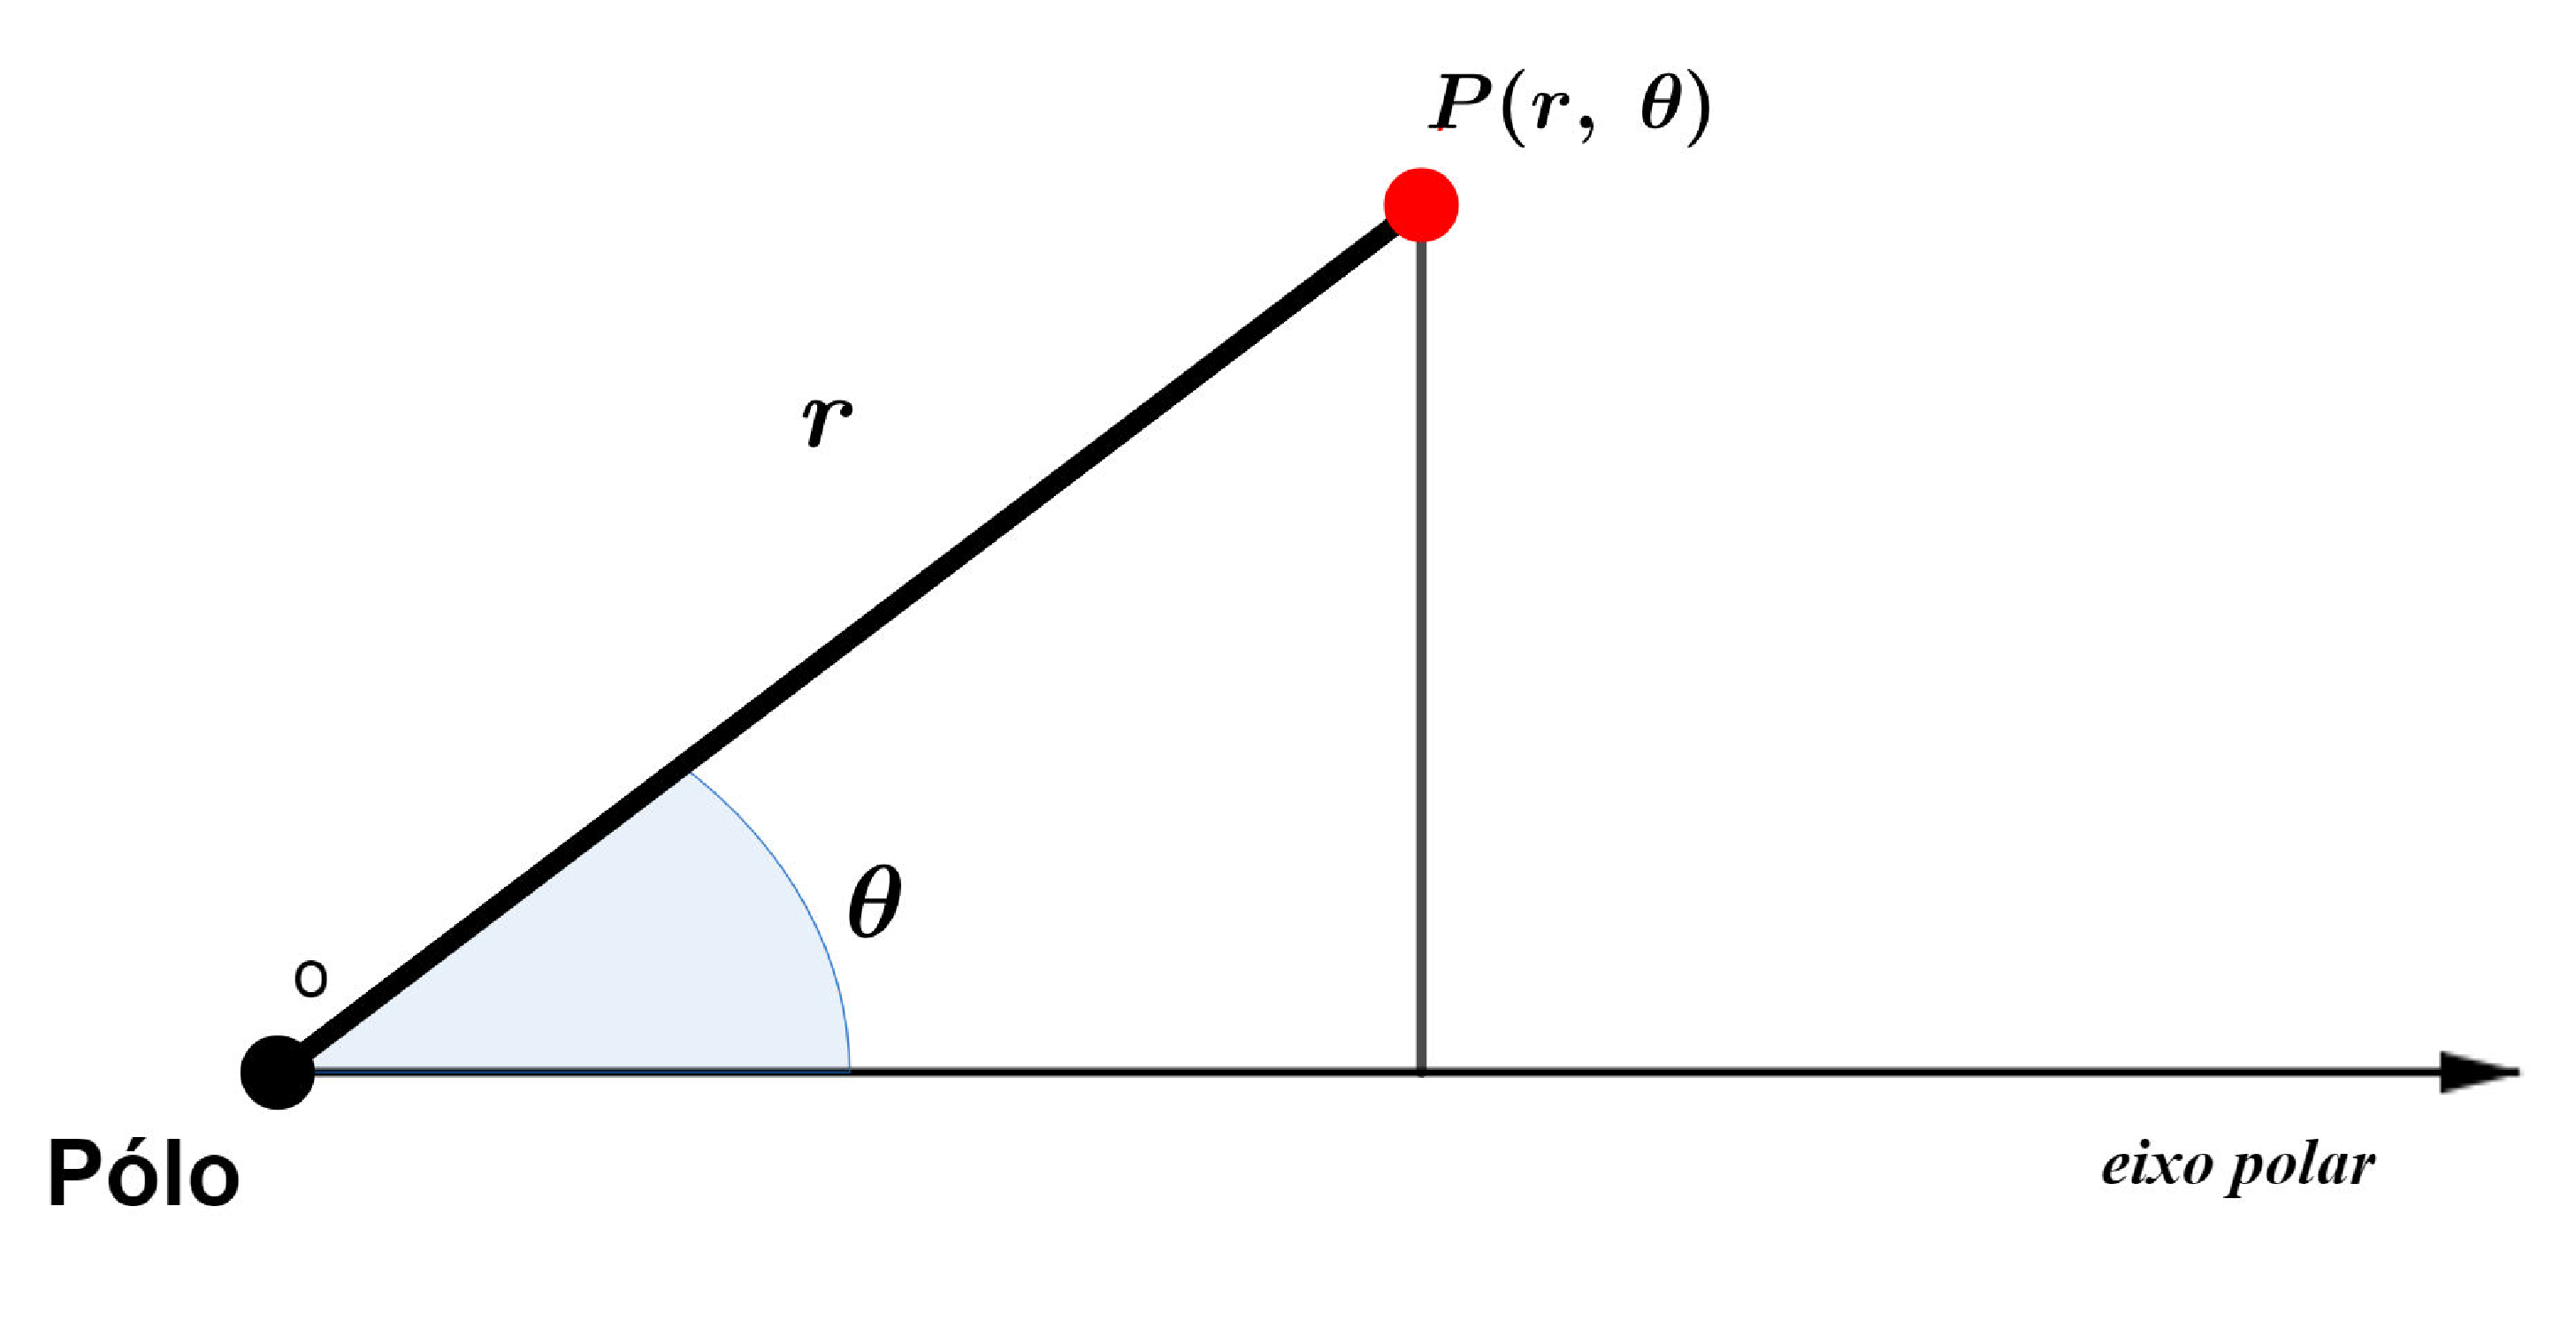
\includegraphics[width=0.4\textwidth]{polar}
	\caption{Sistema de coordenadas polares.}
\end{figure}

É frequente mente útil sobrepor ao sistema de coordenadas polar um sistema de coordenadas retangulares $xy$ de tal forma que o eixo $x$ positivo coincida com o eixo polar. Feito isso, cada ponto $P$ terá coordenadas $(x,y)$, bem como coordenadas polares $(r, \theta)$, conforme a Figura 2, essas coordenadas estão relacionadas pelas equações:

\begin{eqnarray} \label{eq1}
	x = rcos\,\theta, \,\,y = r sen\,\theta
\end{eqnarray}

Dados $r$ e $\theta$, podemos encontar $x$ e $y$, embora para encontrar $r$ e $\theta$ é preferível utilizar as identidades $sen^2\theta$ $+$ $cos^2\theta$ = 1 e tg$\theta$ = sen$\theta$/cos$\theta$ para reescrevermos \eqref{eq1} como:

\begin{center}
	$r^2 = x^2 + y^2, \,\,\,tg\,\theta = \frac{y}{x}$
\end{center}

\begin{figure}[h!]
	\centering
	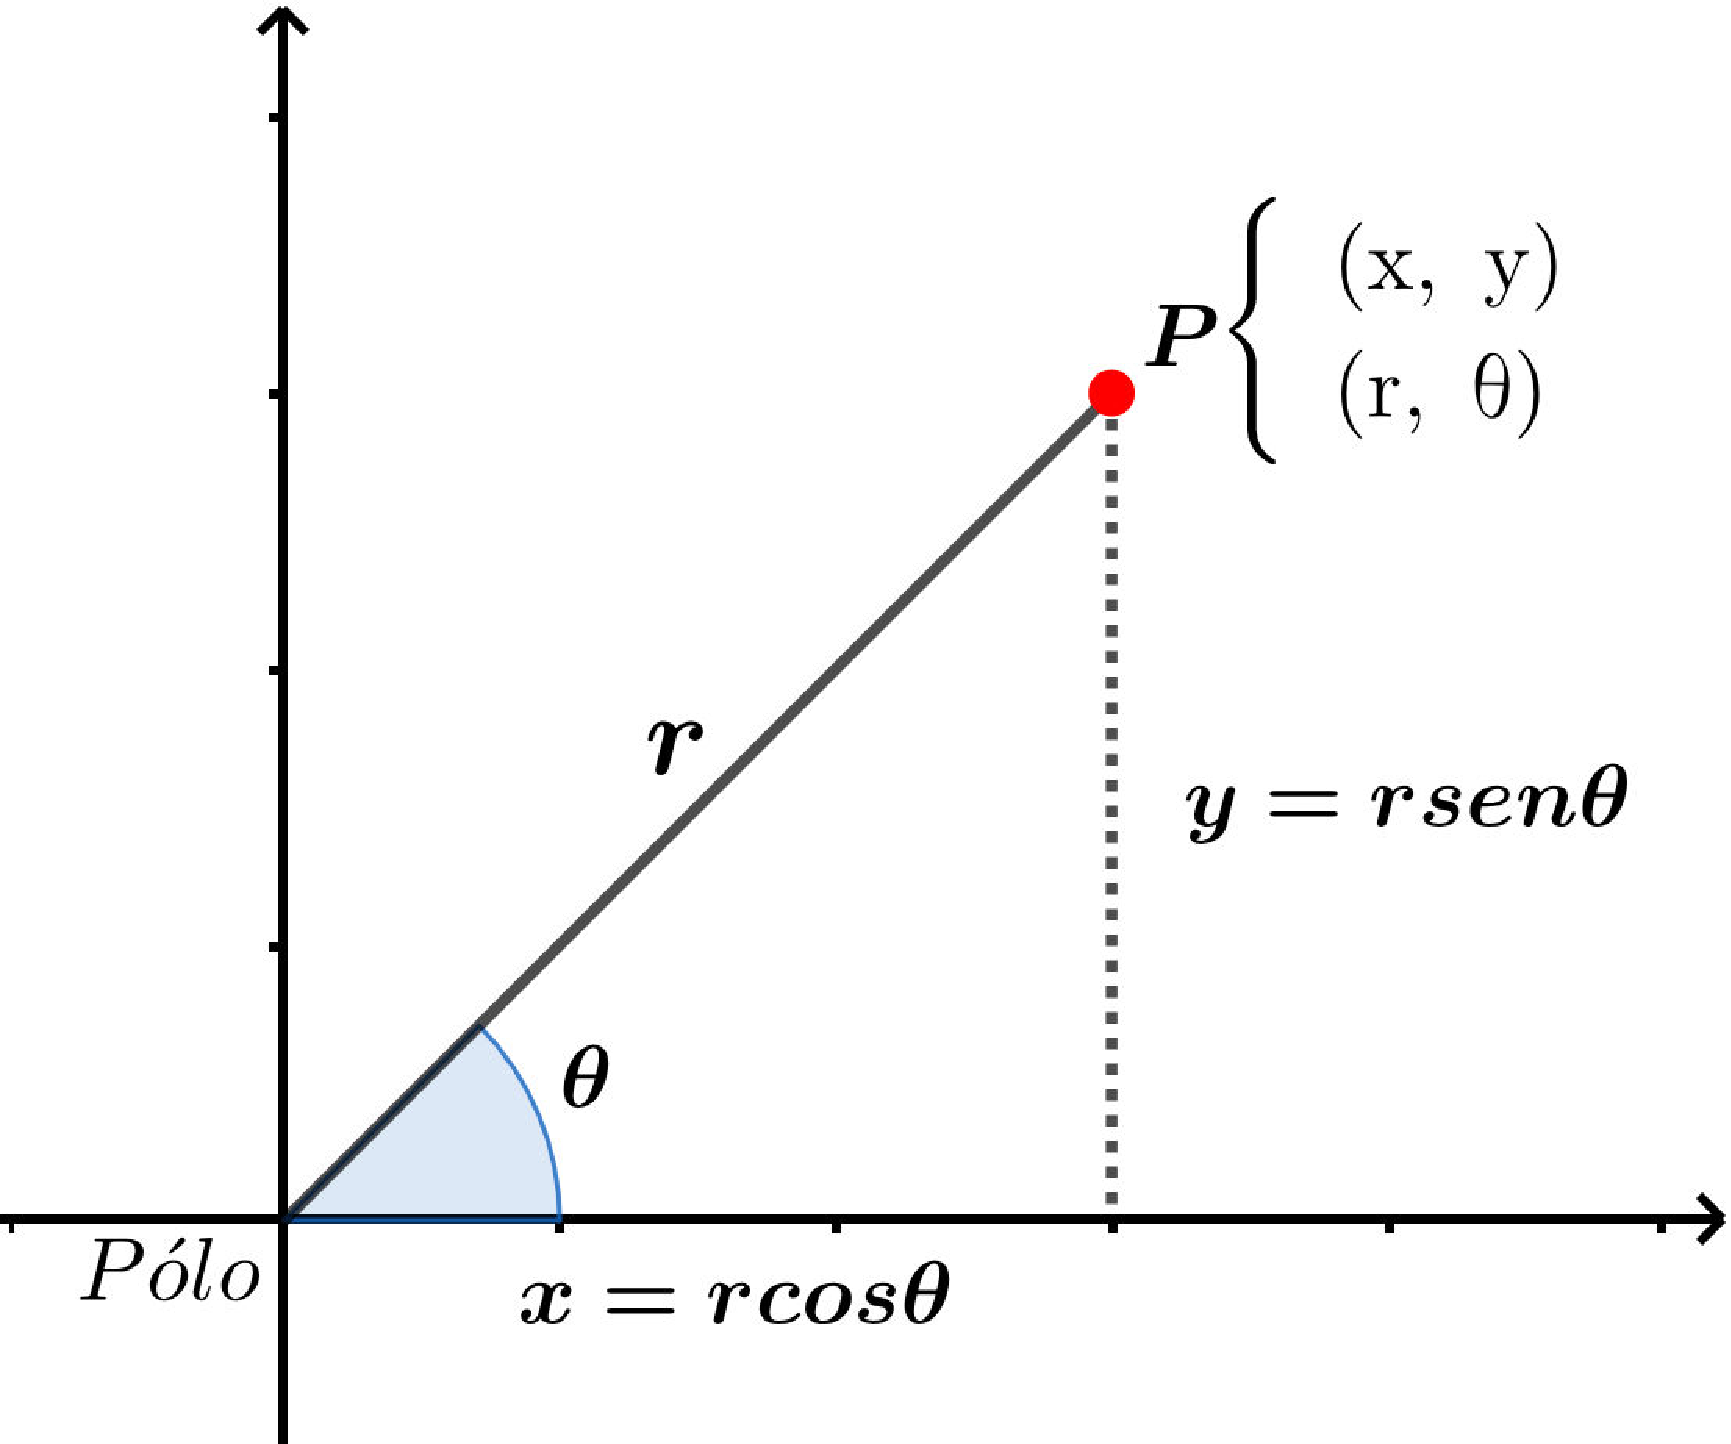
\includegraphics[width=0.3\textwidth]{p1}
	\caption{Relação polar - cartesiano}
\end{figure}

Uma curva no plano é descrita dando-se as coordenadas de seus pontos como funções de uma variável independente.\\

\begin{mydef}
	Uma \it{curva parametrizada diferenciável} do plano é uma aplicação diferenciável $\alpha$ de classe $C^{\infty}$, de uma intervalo aberto $I \subset \R$ em $\R^2$. A variável $t$ $\in I$ é dita parâmetro da curva, e o subconjunto de $\R^2$ dos pontos $\alpha$($t$), $t$ $\in I$, é chamado traço da curva.
	Observamos que uma curva parametrizada diferenciável do plano é uma aplicação $\alpha: I \rightarrow$ $\R^2$ que para cada $t$ associa $\alpha$($t$) $=$ $(x(t)$, $y(t))$, onde as funções $x(t)$ e $y(t)$ são diferenciáveis classe $C^{\infty}$.
\end{mydef}

\textbf{Exemplo:}\\

A aplicação $\alpha(t) = (x_{0}+at, y_{0}+bt), t \in \R$ onde $a^2 + b^2 \neq 0$, é uma curva parametrizada diferenciável cujo traço é uma linha reta, passando pelo ponto $(x(t)$, $y(t))$, paralela ao vetor de coordenadas (a, b) (ver Figura 3).

\begin{figure}[h!]
	\centering
	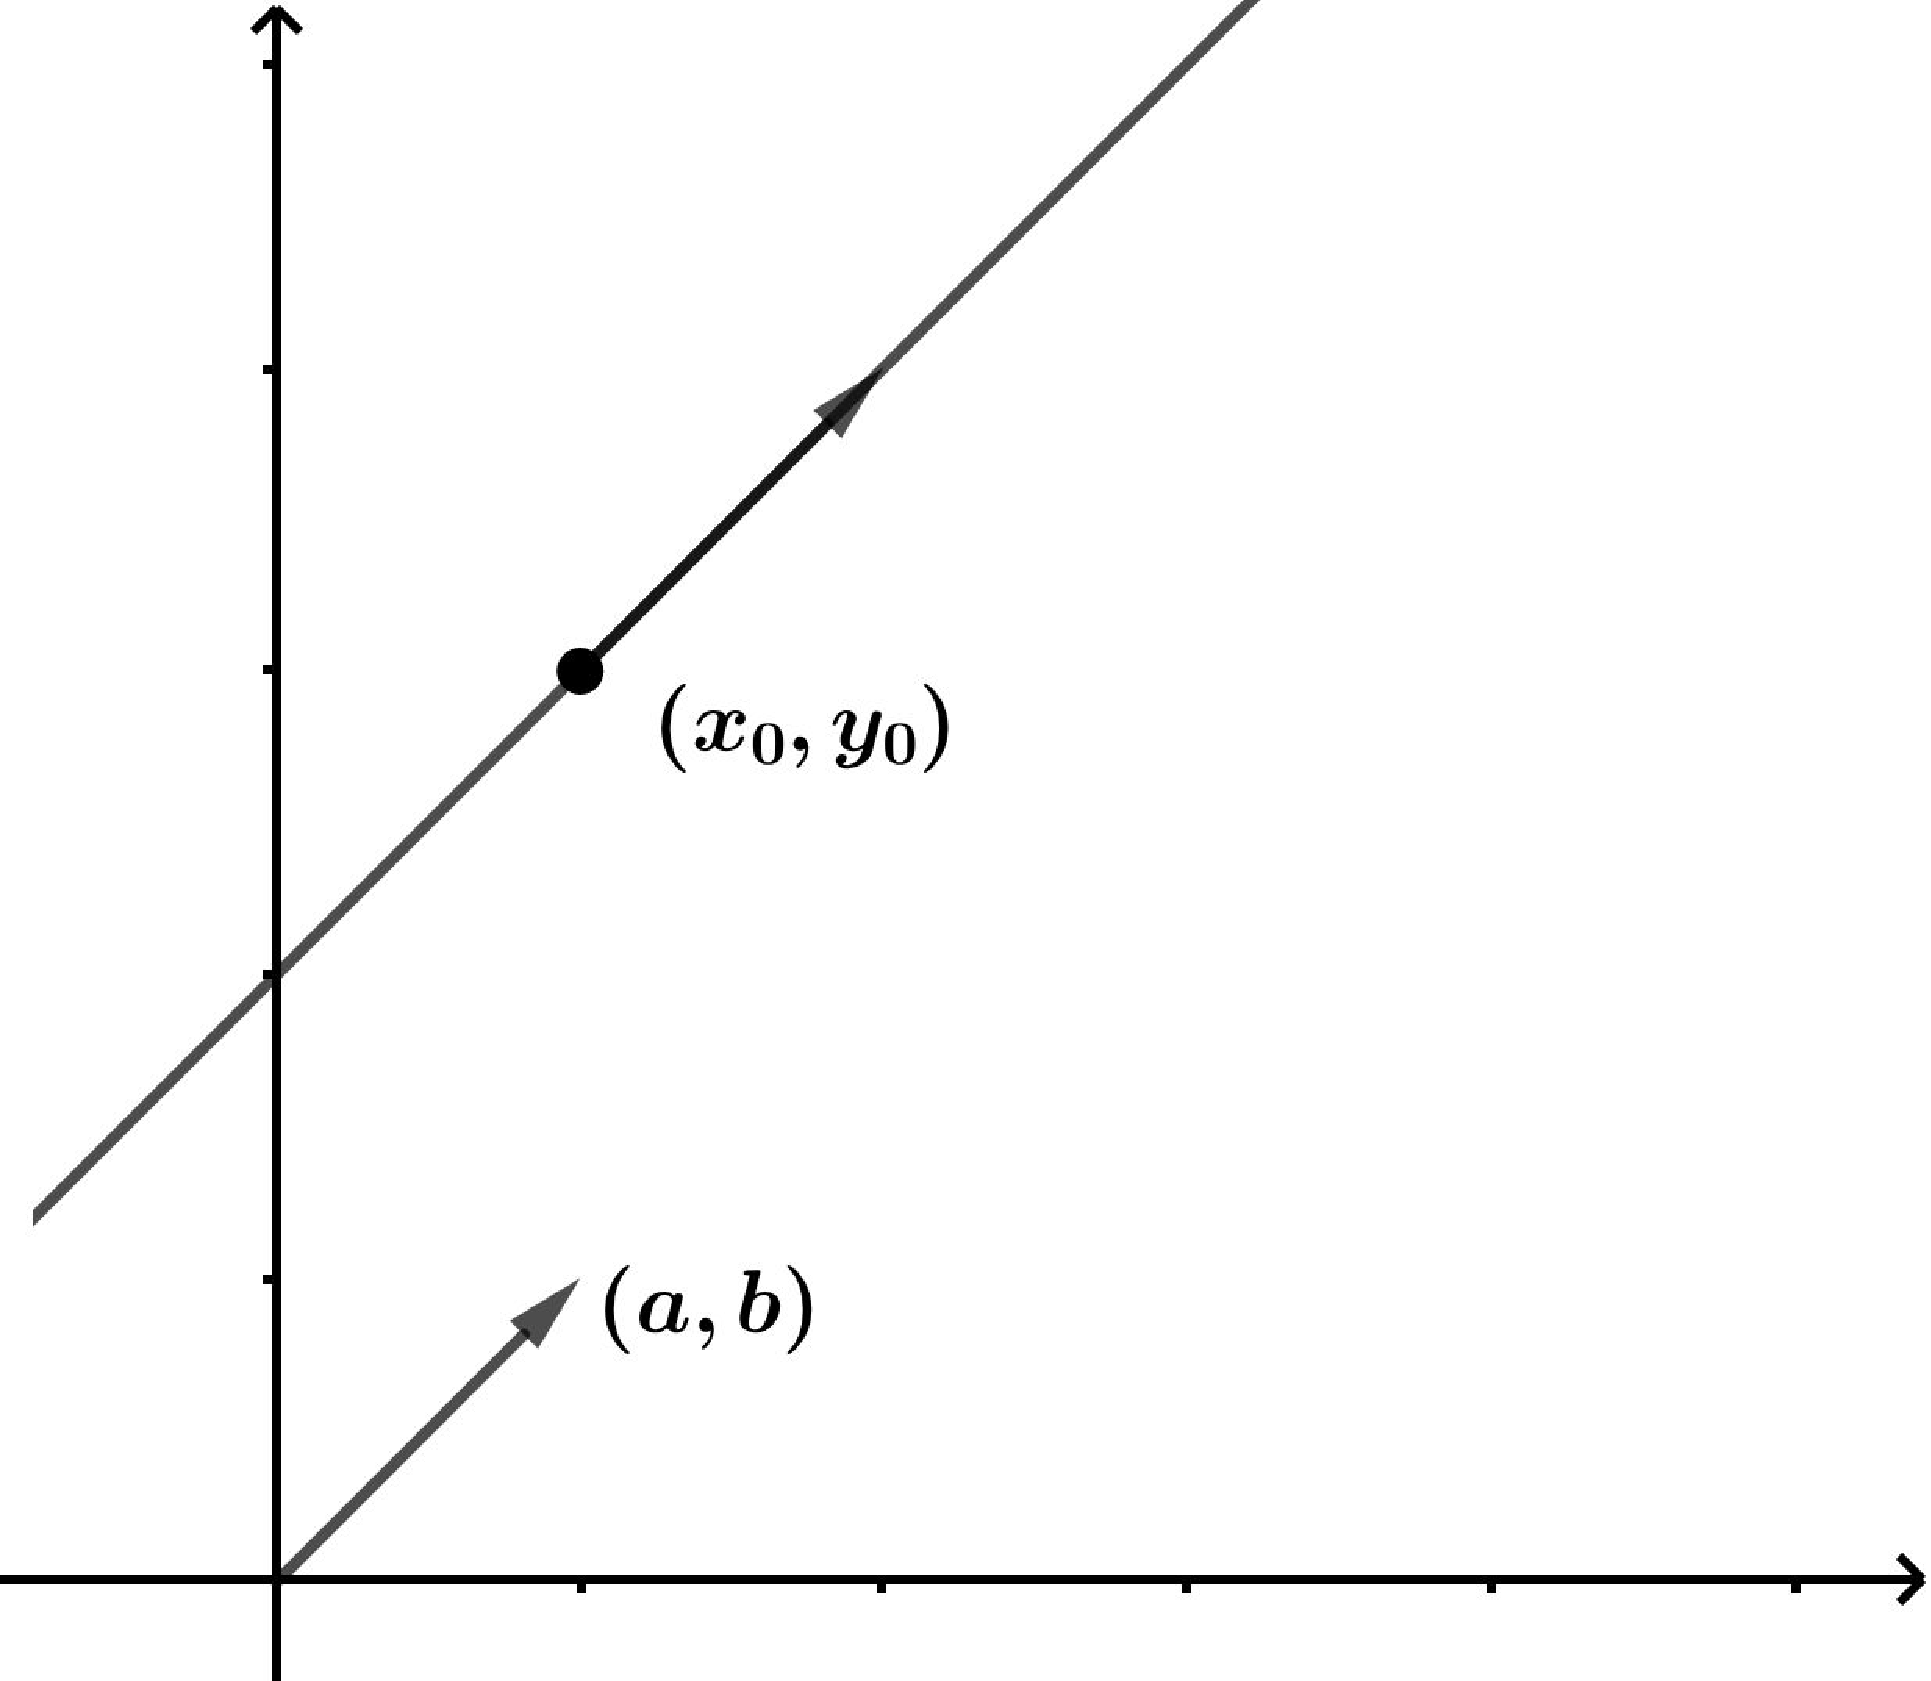
\includegraphics[width=0.3\textwidth]{p2}
	\caption{Reta $\alpha(t)$ que passa por $(x_{0},$ $y_{0})$, na direção de $(a,\,b)$}
\end{figure}

\emph{Abaixo apresentamos outras definições:}\\ \\

A Parametrização descreve o sentido do percurso, então é possível observar um ponto $P$ percorrendo um caminho que, neste caso, é a nossa curva regular $\alpha$. Também, $\alpha$ pode ser vista como uma função, tal que:

\begin{center}
	$I \rightarrow \R^2$ \\ $\alpha(t) = (x(t), y(t))$
\end{center}

Observando que nem sempre $\alpha$ é o gráfico de $t$, de modo que a trajetória é a imagem da função $\alpha$ em relação a $t$. Então, os pontos pelos quais $P$ passa na trajetória formam sua imagem. Sendo assim, é possível obter uma equação cartesiana para a parametrização da curva, onde todos os pontos da função estão contidos na equação. Ex: $\alpha(t) = (1+3t , 2+t); t\in \mathbb{R}$ (ver Figura 4).

\begin{figure}[h!]
	\centering
	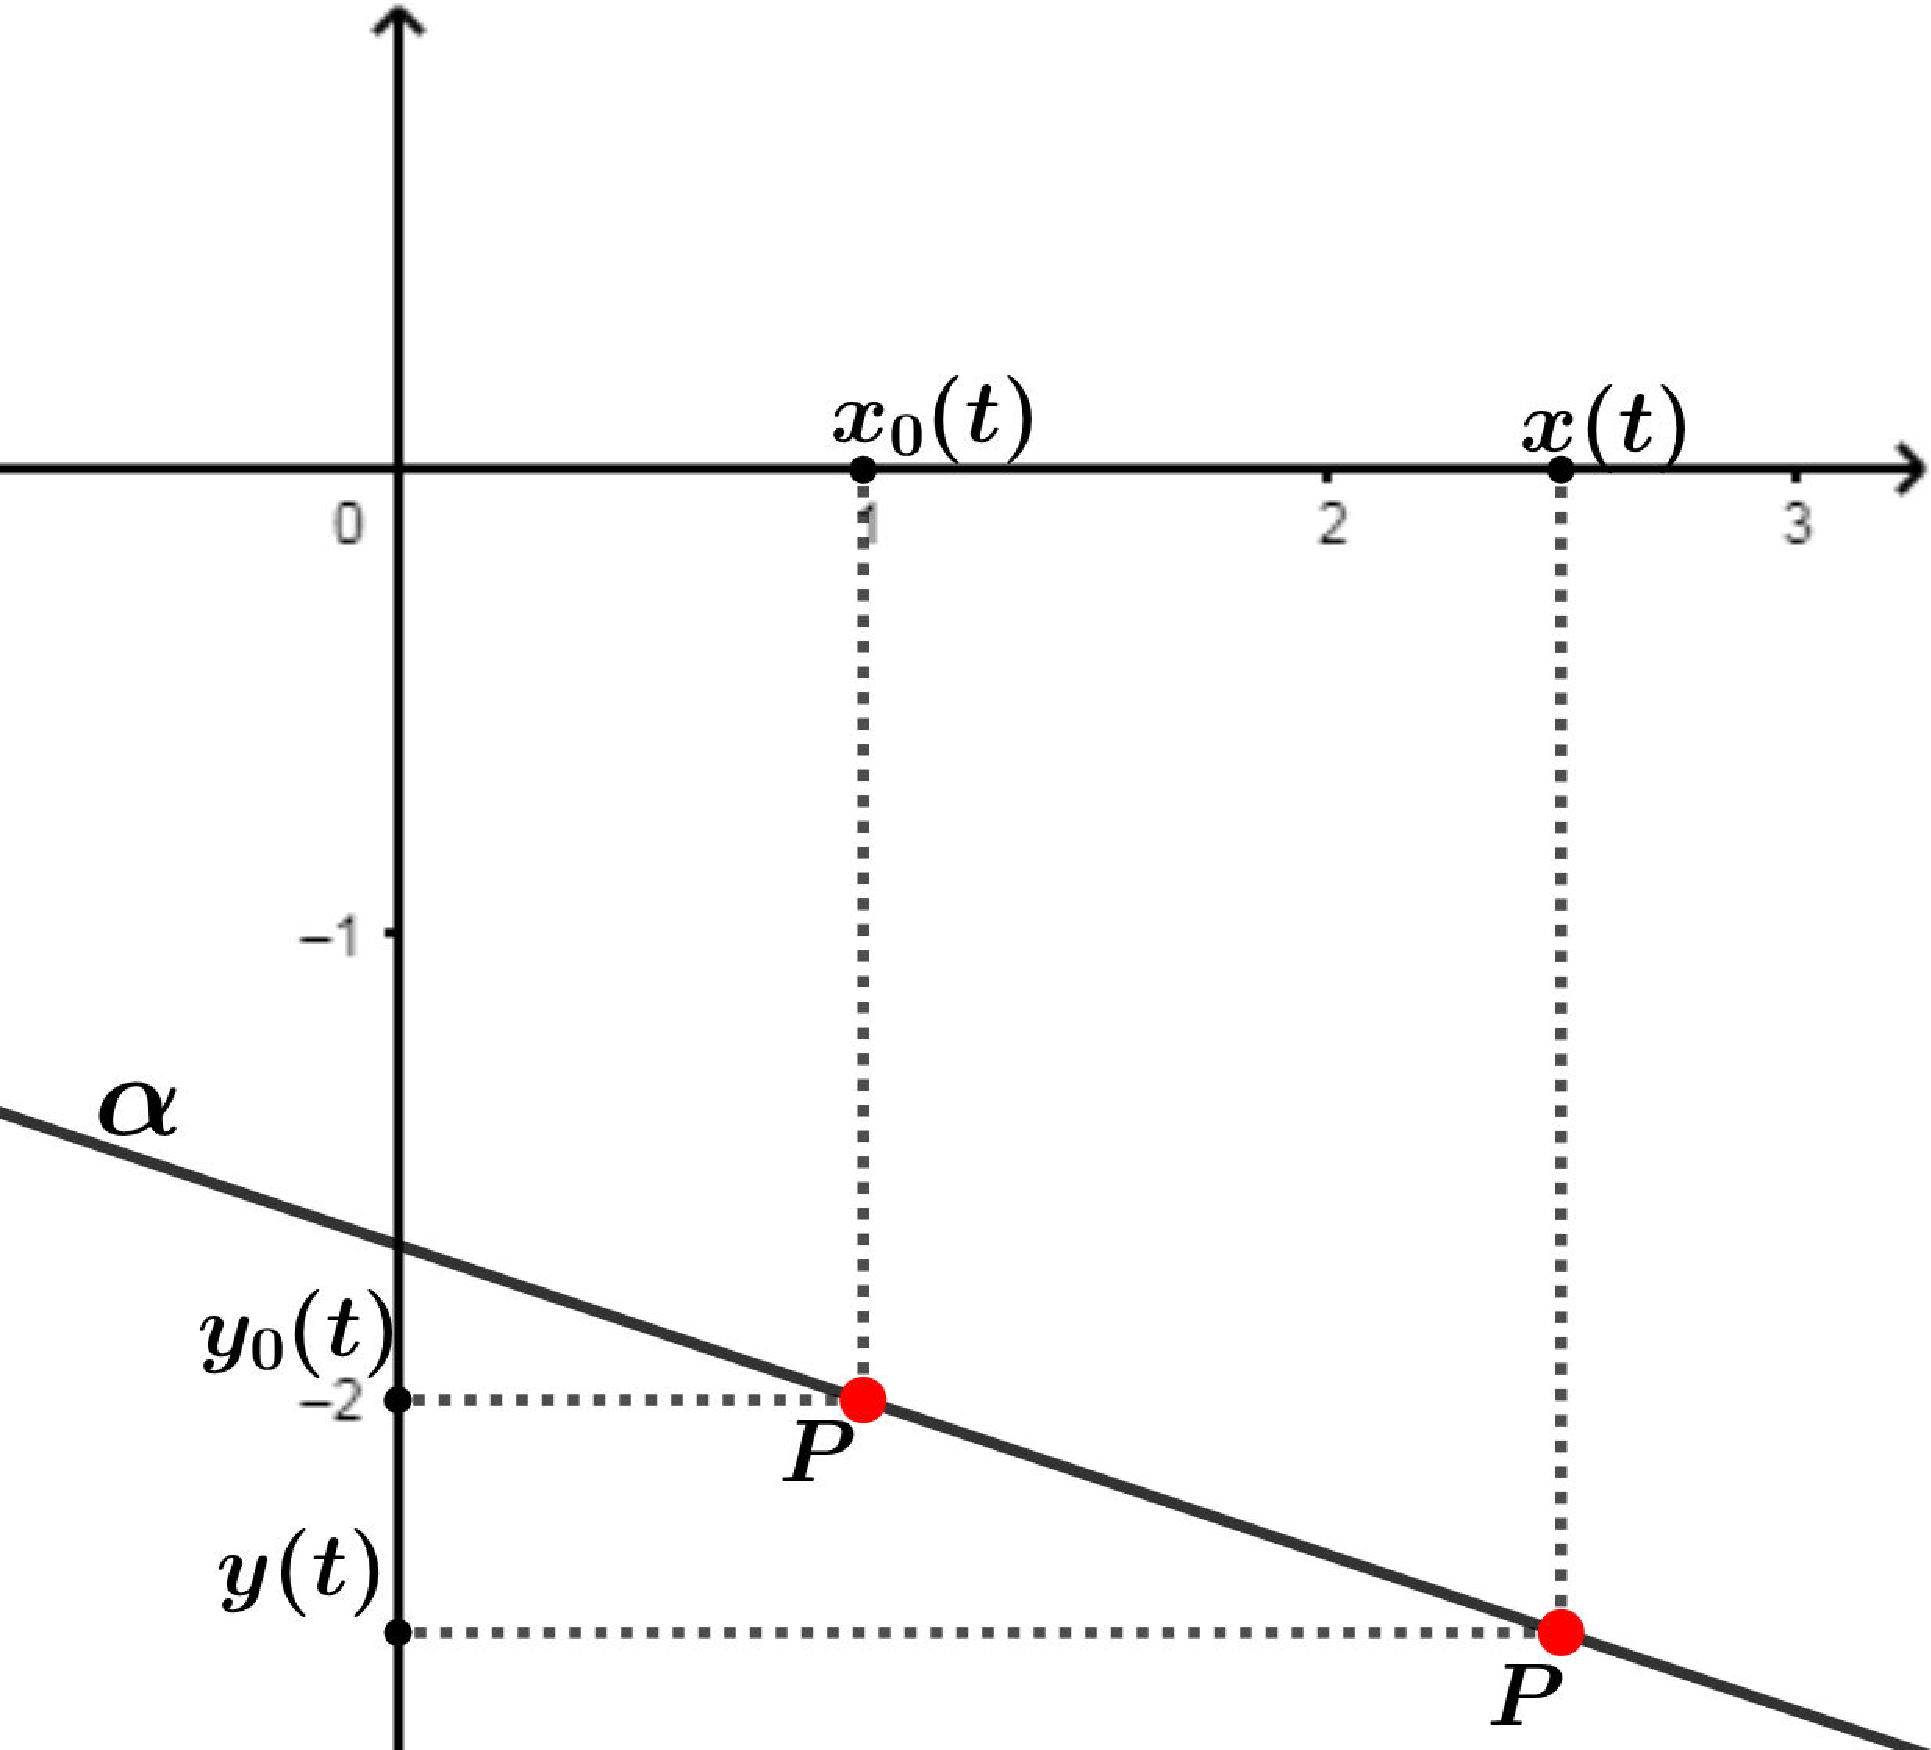
\includegraphics[width=0.3\textwidth]{alpha}
	\caption{Traço de $\alpha$}
\end{figure}

O conjunto imagem de $\alpha$ é dado por:

\begin{center}
	{\bf\it C} = $\left\{\alpha(t) = (x(t), y(t)), t\in {\bf\it I} \right\}$
\end{center} 
	
Onde $C$ é chamado traço de $\alpha$. Consequentemente, $\alpha$ é dita uma parametrização de $C$. \section{Espirais}
	
As espirais são curvas planas que giram em torno de um ponto central (chamado pólo), dele se afastando ou se aproximando segundo uma determinada lei. Quando se volta para a direita é chamada espiral dextrógira e quando para esquerda é conhecida como sinistrogira ou levogira. Neste capítulo estarão expostas as espirais mais conhecidas, e em especial a espiral logarítmica e sua inversa.

\subsection{Espiral de Arquimedes}

A espiral de Arquimedes é o conjunto de pontos dado por $E = \left\{(x, y)\, \in \R^{2} \,|\, y = x\,tan\left(\frac{\sqrt[]{x^2 + y^2}}{a}\right)\right\}$ , onde $a$ $>$ $0$. Utilizando coordenadas polares, podemos parametrizar a espiral de Arquimedes: $a\theta, a$ $>$ $0$, sendo $\theta$ em radianos. $\alpha$ $=$ $(a\theta, \theta)$, então podemos escrever a espiral como o traço da curva $\alpha$:$[0, \infty) \rightarrow \R^2$ definida por: (ver Figura 5).

\begin{center}
	$\alpha(t)$ $=$ $(at\,cos(t)$, $at\,sen(t))$, $t\in I$
\end{center}

\begin{figure}[h!]
	\centering
	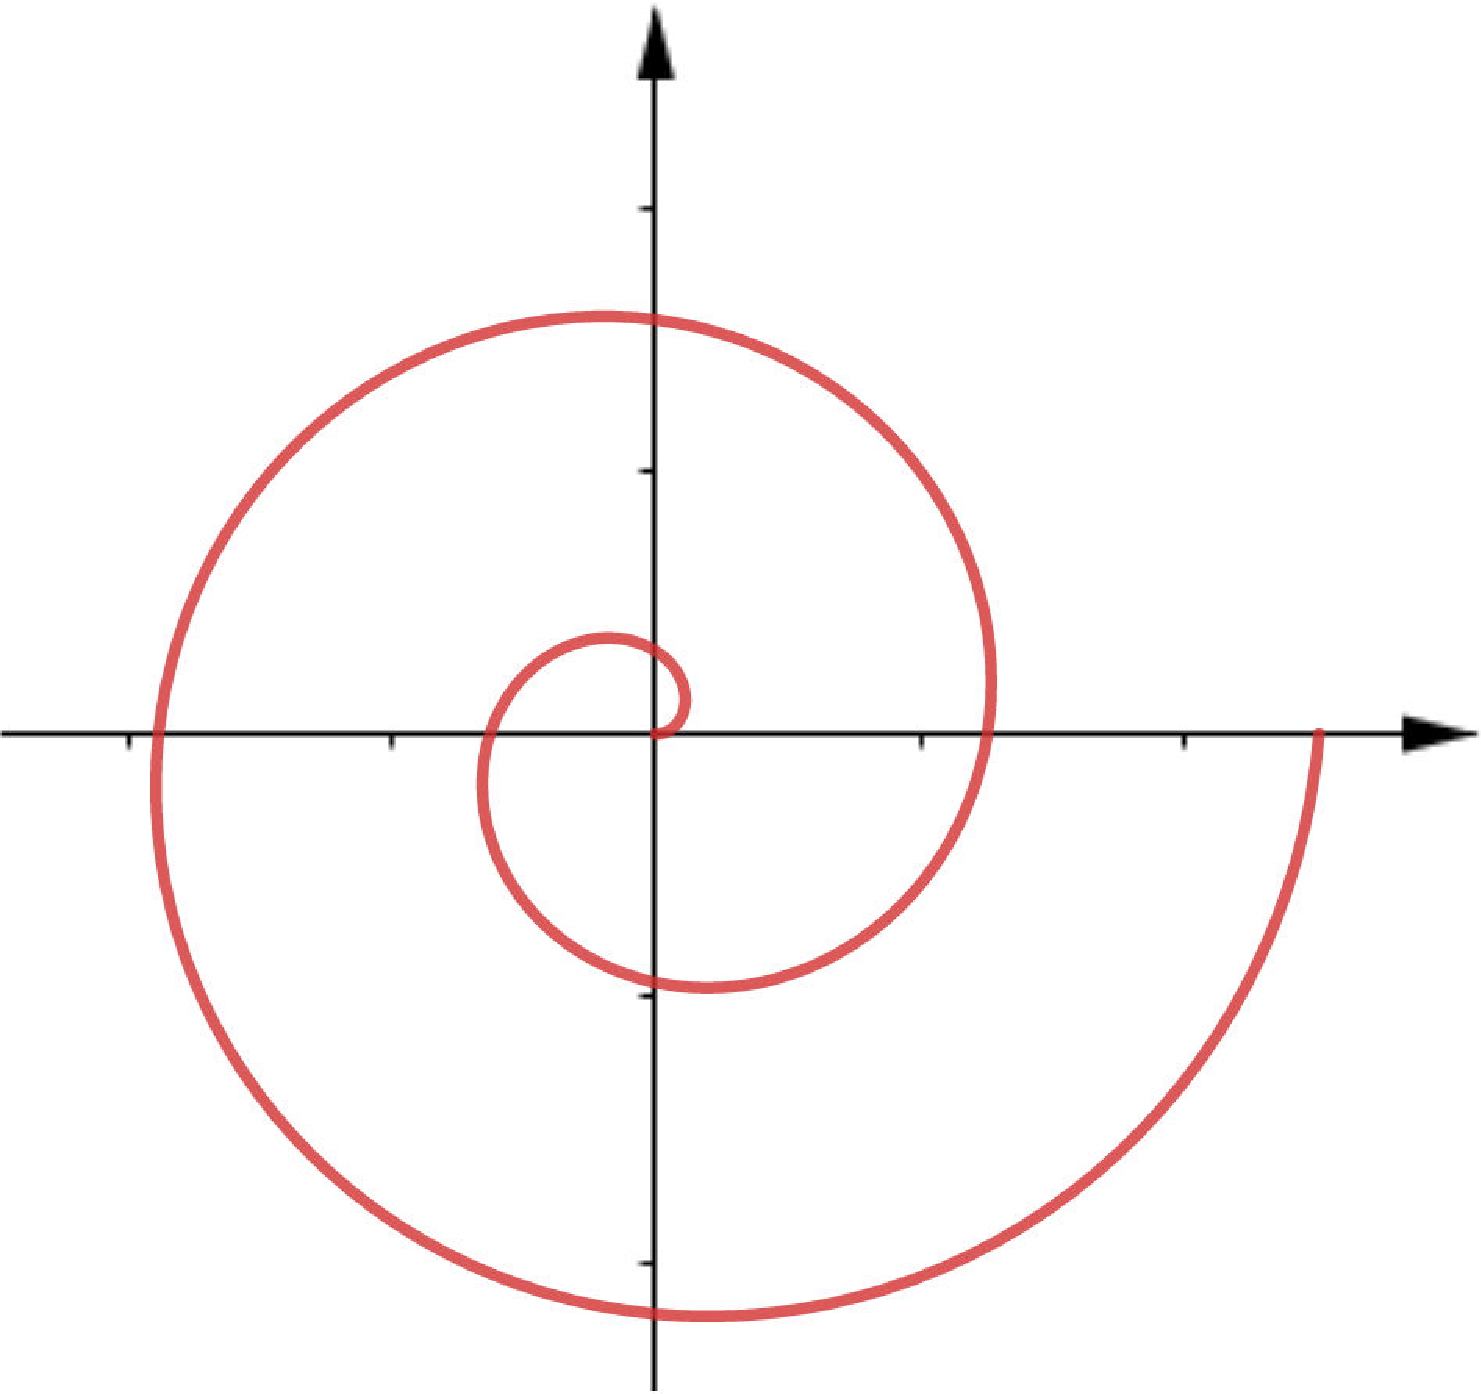
\includegraphics[width=0.3\textwidth]{archim}
	\caption{Traço da espiral de arquimedes.}
\end{figure}

De modo geral, a equação polar de uma espiral arquimediana é da forma: $r$ = $a\theta^{1/n}$, onde a variável $n$ determina o quão encaracolado ela será, quando $n$ $<$ $0$, a espiral tende a ter voltas com valores para $r$, tal que: $-2$ $\leq$ $r$ $\leq$ $2$. No caso da espiral de Lituus, $n$ $=$ $-2$, logo, $r$ $=$ $a\theta^{-1/2}$ ou $r$ $=$ $\frac{a}{\sqrt[]{\theta}}$. Os valores de $r$, quando $\theta$ assume valores próximos de $0$, o gráfico de $r$ $=$ $a\theta^{-1/2}$ tende a formar um setor circular. Como $\alpha = \left(\frac{a}{\sqrt[]{\theta}}, \theta\right)$, logo sua parametrização $\alpha$: $[0, \infty) \rightarrow \R^2$ é definida como: (ver Figura 6).

\begin{center}
	$\alpha(t) = \left(\frac{a}{\sqrt[]{t}}\,cos(t), \frac{a}{\sqrt[]{t}}\,sen(t)\right)$, $t\in I$
\end{center}

\begin{figure}[h!]
	\centering
	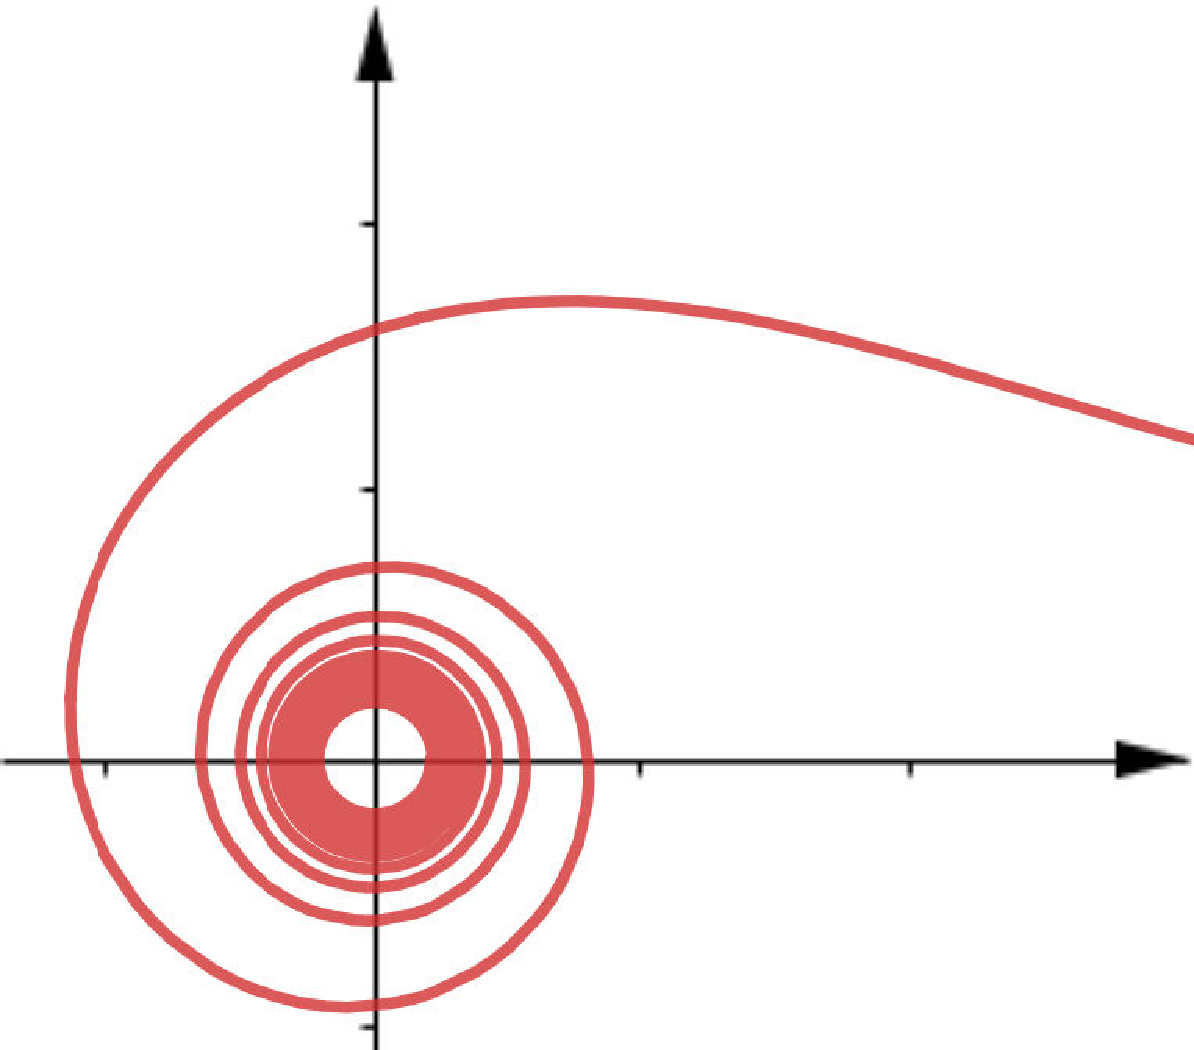
\includegraphics[width=0.3\textwidth]{lituus}
	\caption{Traço da espiral de Lituus}
\end{figure}

\subsection{Espiral de Fermat}

A equação da espiral de Fermat, ou espiral parabólica, é uma espiral arquimediana que possui equação em coordenadas polares: $r$ $=$ $a\,\theta^{1/n}$, onde $n$ $=$ $2$, logo teremos $r$ = $a\theta^{1/2}$. Esta espiral para qualquer valor de $\theta$ $>$ $0$ obtemos dois correspondentes a $r$, mas de sinais opostos, sendo $r$ $=$ $a\theta^{1/2}$ e $r$ $=$ $-a\theta^{1/2}$. Tomando ambos os sinais das espirais obtemos espirais simétricas em relação à origem (ver figura 7).

\begin{figure}[h!]
	\centering
	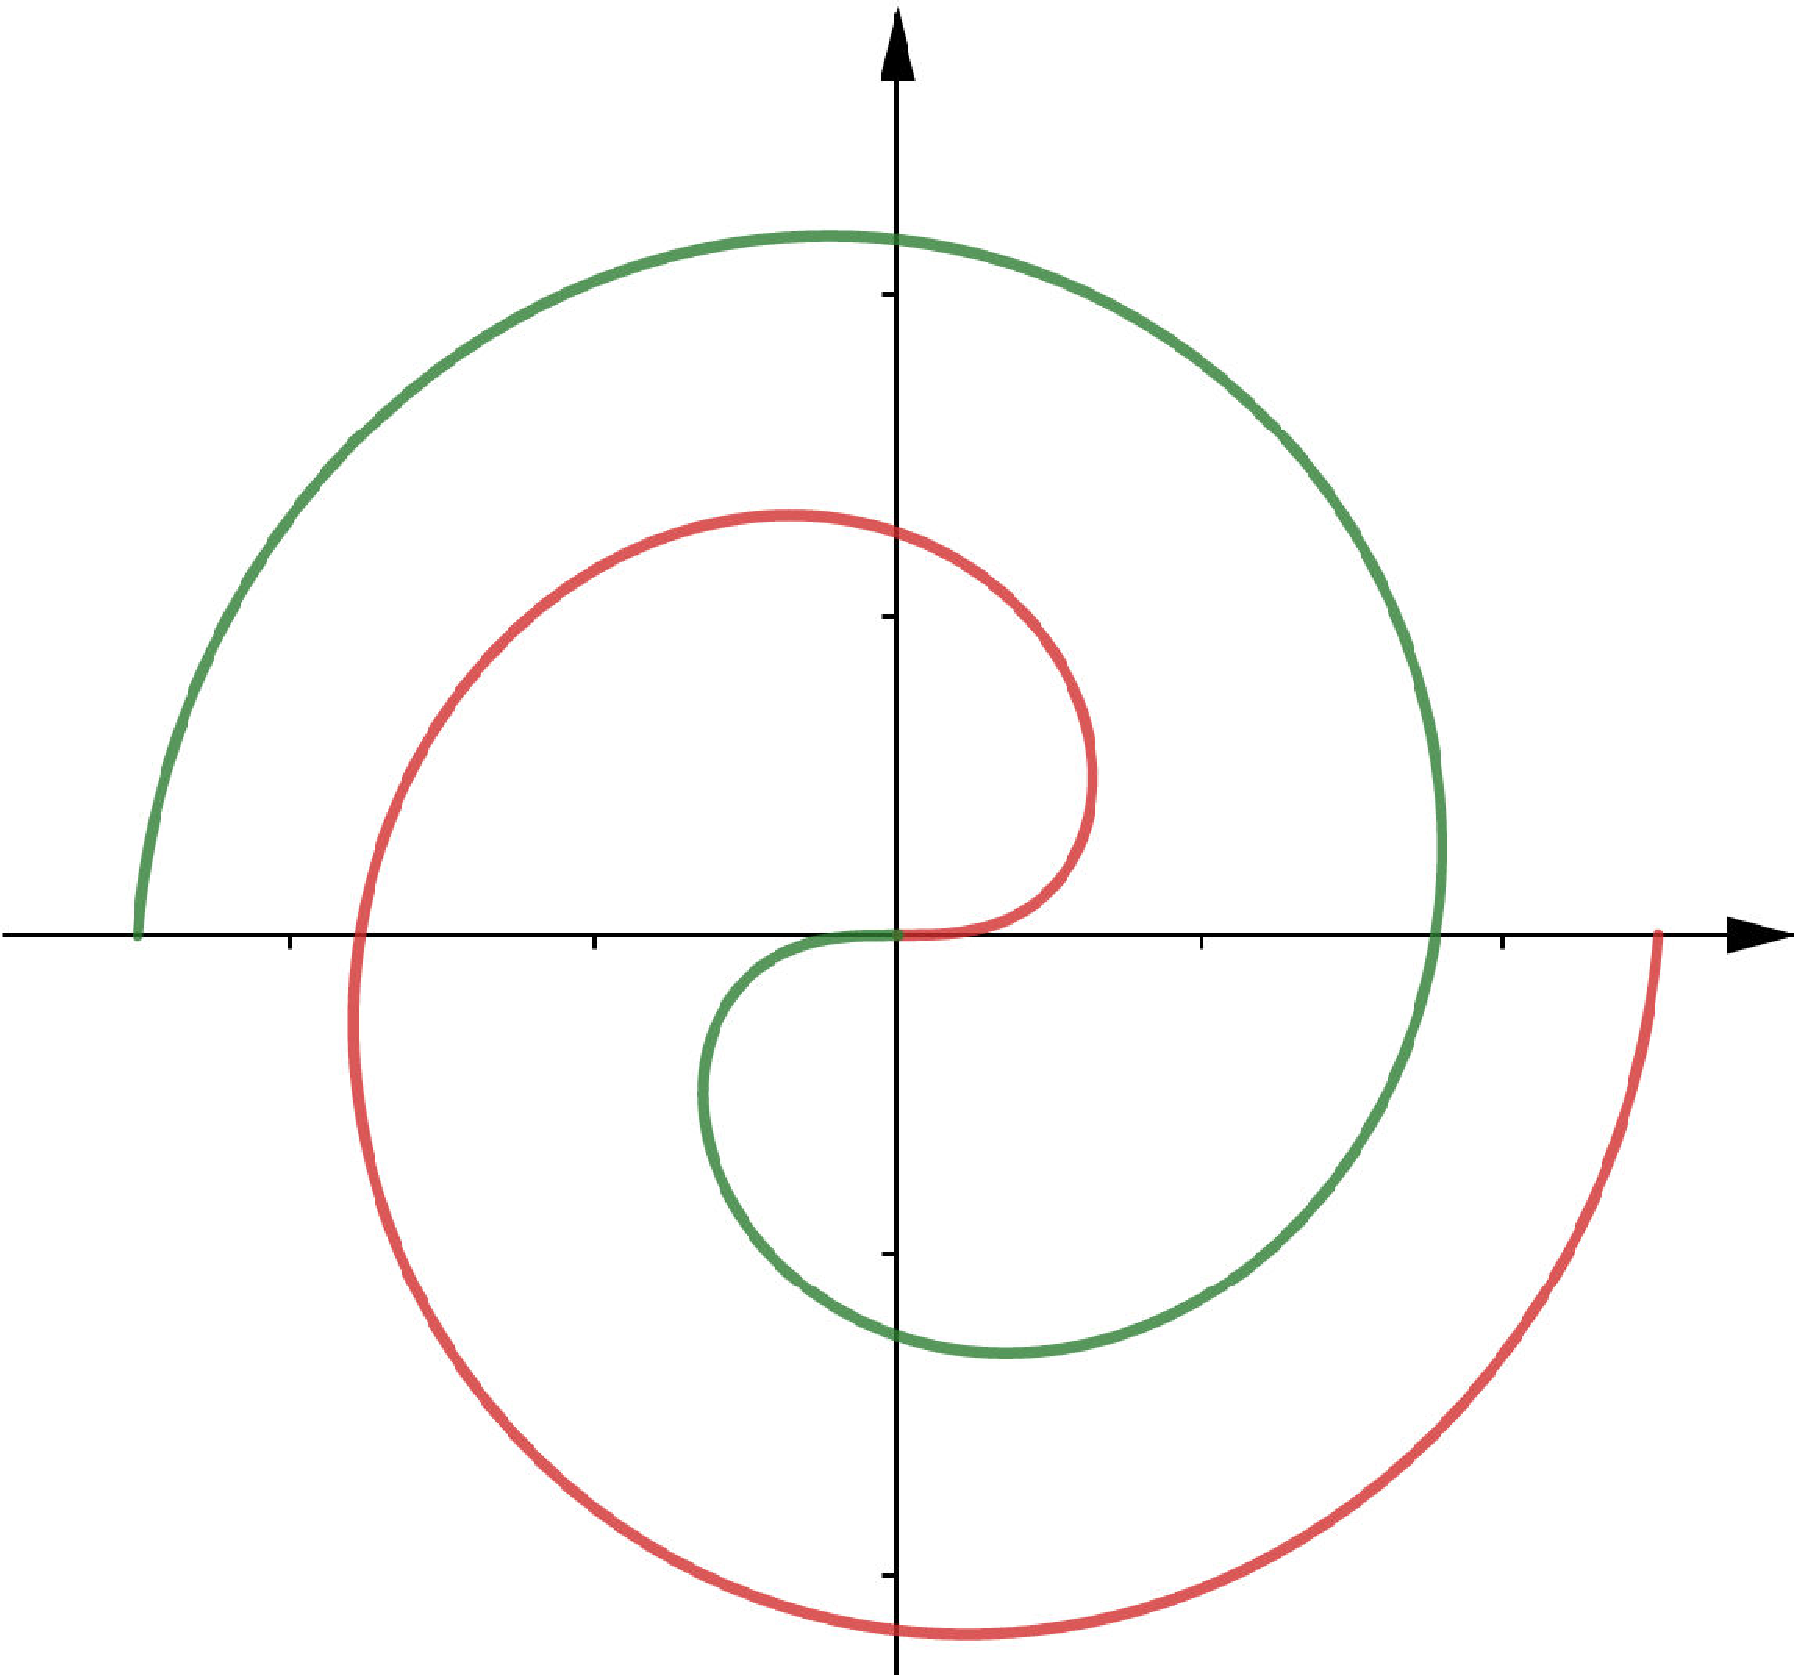
\includegraphics[width=0.3\textwidth]{fermat}
	\caption{Gráfico da espiral de Fermat}
\end{figure}

\subsection{Espiral hiperbólica}

A espiral hiperbólica, é a espiral inversa da espiral de Arquimedes. Assim como a espiral de Lituus, começa em uma distância infinita em relação ao eixo das ordenadas, e se enrola cada vez mais rapidamente a medida que se aproxima da origem. Em coordenada polar temos: $r$ $=$ $a\theta^{-1}$, logo também é uma arquimediana, com $n$ $=$ $-1$. Diferente de outras espirais em que os intervalos partem de $[0, \infty) \rightarrow \R^2$, seu intervalo é contrário devido a sua natureza, logo $\alpha:$ $(\infty, 0] \rightarrow \R^2$ e tem traço descrito por (ver figura 8):

\begin{center}
	$\alpha(t)$ $=$ $(a\frac{cos(t)}{t},$ $a\frac{sen(t)}{t})$, $t\in I$
\end{center}

\begin{figure}[h!]
	\centering
	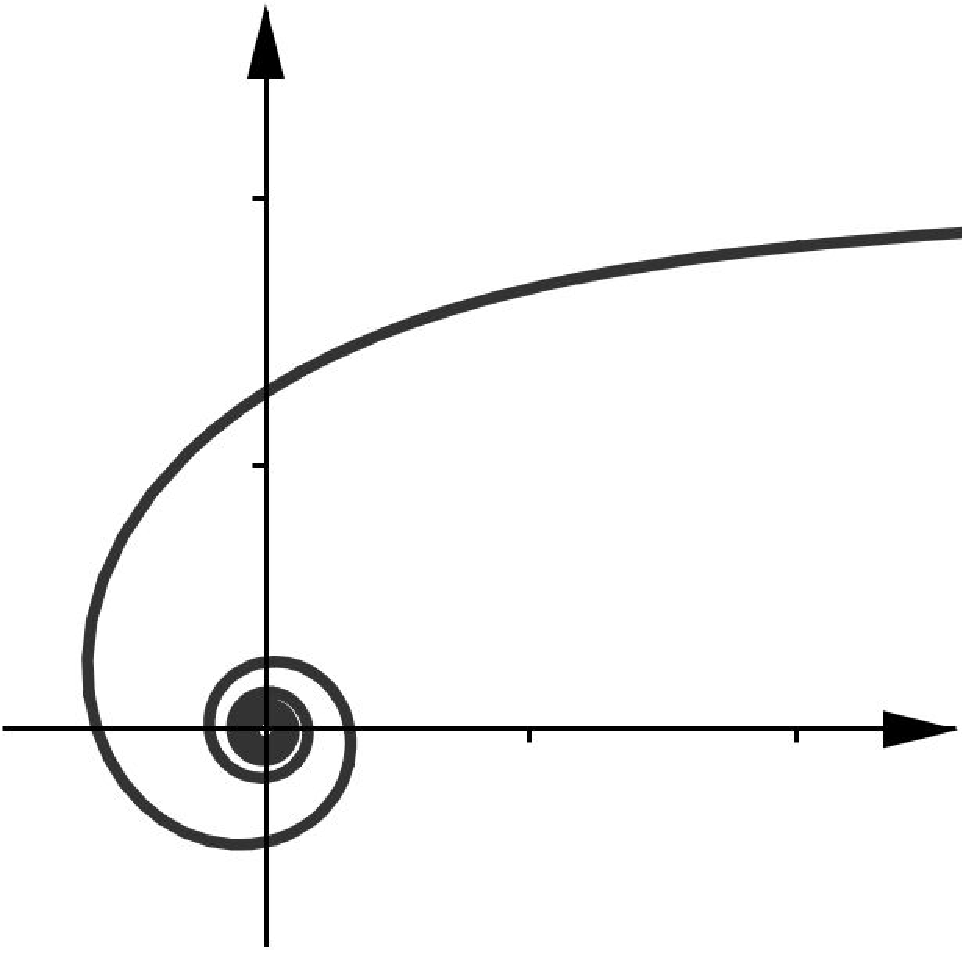
\includegraphics[width=0.3\textwidth]{hiper}
	\caption{Traço da espiral hiperbólica}
\end{figure}

\subsection{Espiral Logarítmica}

A espiral logarítmica foi estudada pela primeira vez por Descartes, e então por Jacob Bernoulli (1654 – 1705), que chamou a curva de $spira$ $mirabilis$ (em latim, espiral maravilhosa), essa curva possui relação com a sequência de Fibonacci e também a proporção áurea. Tem sido tradicionalmente escolhida para descrever os traços dos membros de galáxias espirais, pois, seus "braços" \, são aproximadamente espirais logarítmicas. O nome da espiral logarítmica tem a sua origem na sua lei de formação, em coordenada polar temos: $r = Re^{\theta\,cot\,\alpha}$, mas para sua paramétrica utilizará sua simplificada, $r = a\,e^{b\,\theta}$. Então definimos, $\alpha$ $=$ $( a\,e^{b\,\theta}$, $\theta)$, com intervalo definido $[0, \infty) \rightarrow \R^2$, podemos formar o conjunto imagem de $\alpha(t)$ dado por (ver figura 9):\\

\begin{center}
	$\alpha(t)$ $=$ $(a\,cos(t)\,e^{b\,t},$ $a\,sen(t)\,e^{b\,t})$, $t\in I$
\end{center}

\begin{figure}[!h]
	\centering
	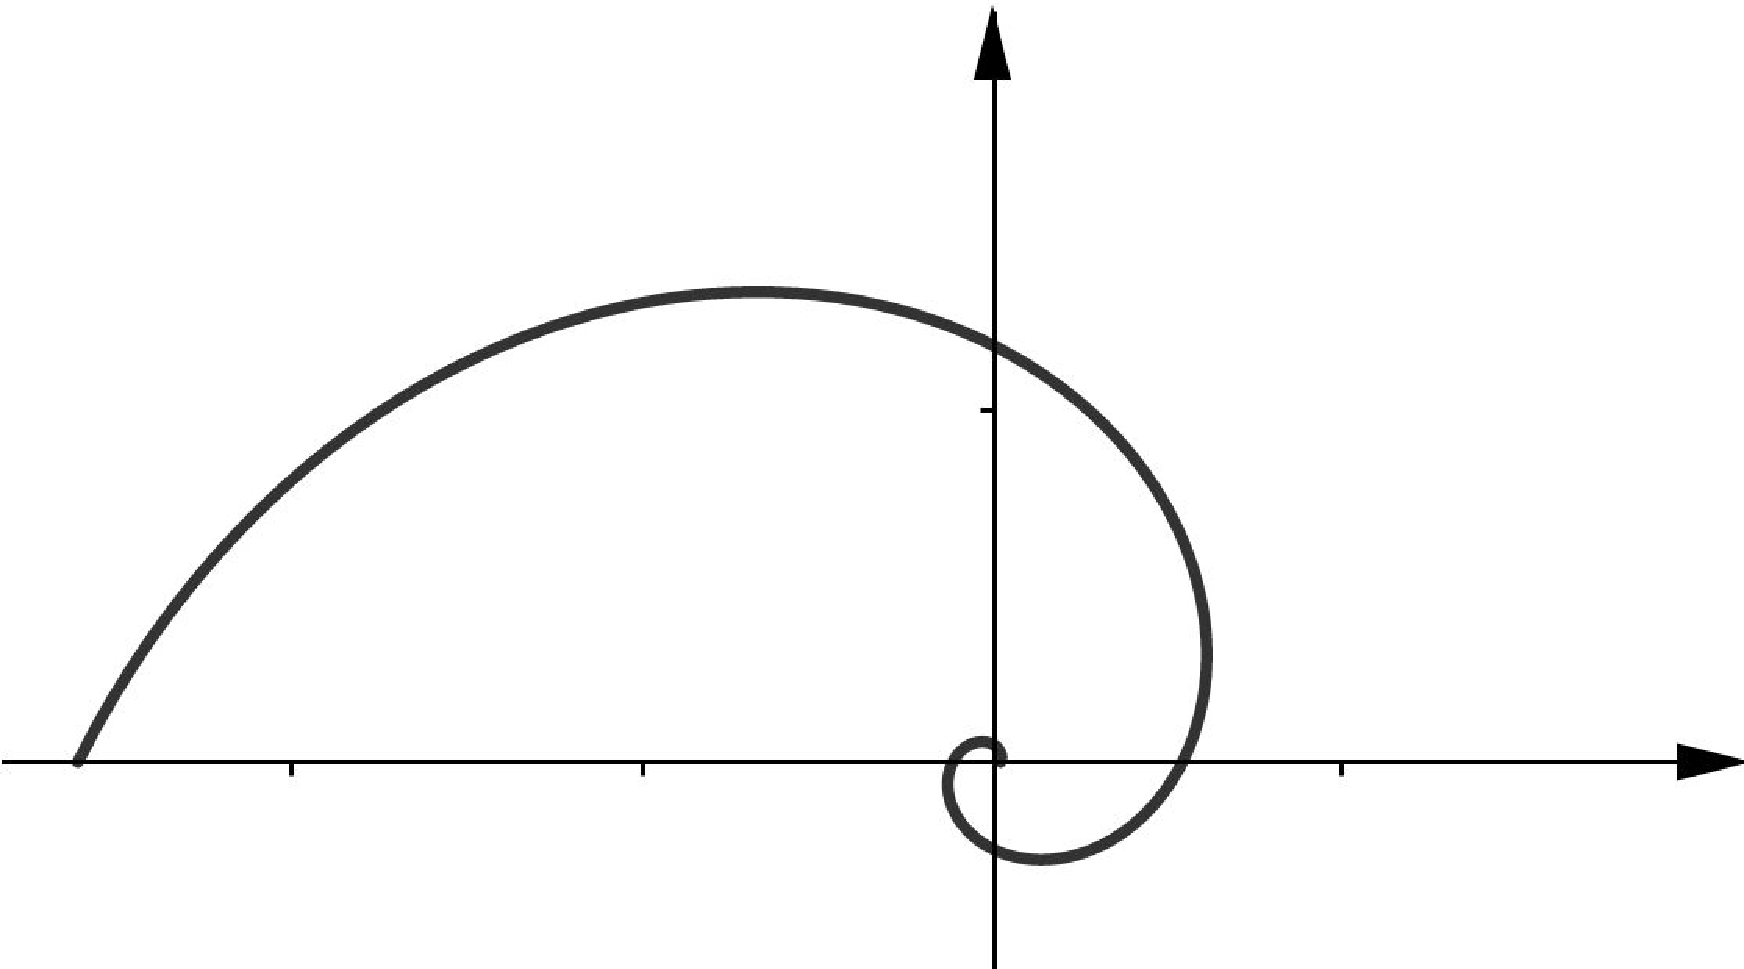
\includegraphics[width=0.3\textwidth]{log}
	\caption{Traço da espiral logarítmica}
\end{figure}

Porém, outra fórmula deriva da análise de equações encontrada na geometria não-euclidiana de espaços negativamente curvados. Esta geometria hiperbólica foi descoberta e publicada por Bolyai (1832) e independentemente por Lobachevsky. Essa nova fórmula foi descoberta por Harry I. Ringermarcher e Lawrence R. Mead, no artigo publicado em 2009 “A New Formula Describing the Scaffold Structure of Spiral Galaxies”, descrevendo com maior perfeição os membros de uma galáxia espiral. Em coordenada polar temos:

\begin{align*}
	r(\theta) = \frac{A}{log\left(B\,tan\,\frac{\theta}{2N}\right)}
\end{align*}
 
Onde $A$ é uma parâmetro de escala para toda estrutura enquanto $B$ e $N$ determina a curvatura da espiral. Definindo $[0, \infty) \rightarrow \R^2$, teremos o seguinte conjunto:

\begin{equation} \label{eq2}
	\alpha(t) = \begin{cases}
		x = \frac{A}{log\left(B\,tan\,\frac{t}{2N}\right)}\,cos(t) \\
		y = \frac{A}{log\left(B\,tan\,\frac{t}{2N}\right)}\,sen(t)
	\end{cases} 
\end{equation}

A partir desta parametrização obteremos os traços dos membros de diferentes formações, proeminentes da manipulação das variáveis $A$, $B$, e $N$, delimitando quando conveniente o intervalo de crescimento das curvas, pois, como experimento vamos pegar curvas de intervalos finitos, para assim sobrepor imagens de galáxias e verificar o comportamento dessas curvas sob as imagens ilustrativas. Alguns exemplos de curvas com $A = 1$:

\begin{figure*}[!h]
	\centering
	\subfigure[$B = 0.25, N = 7$]
		{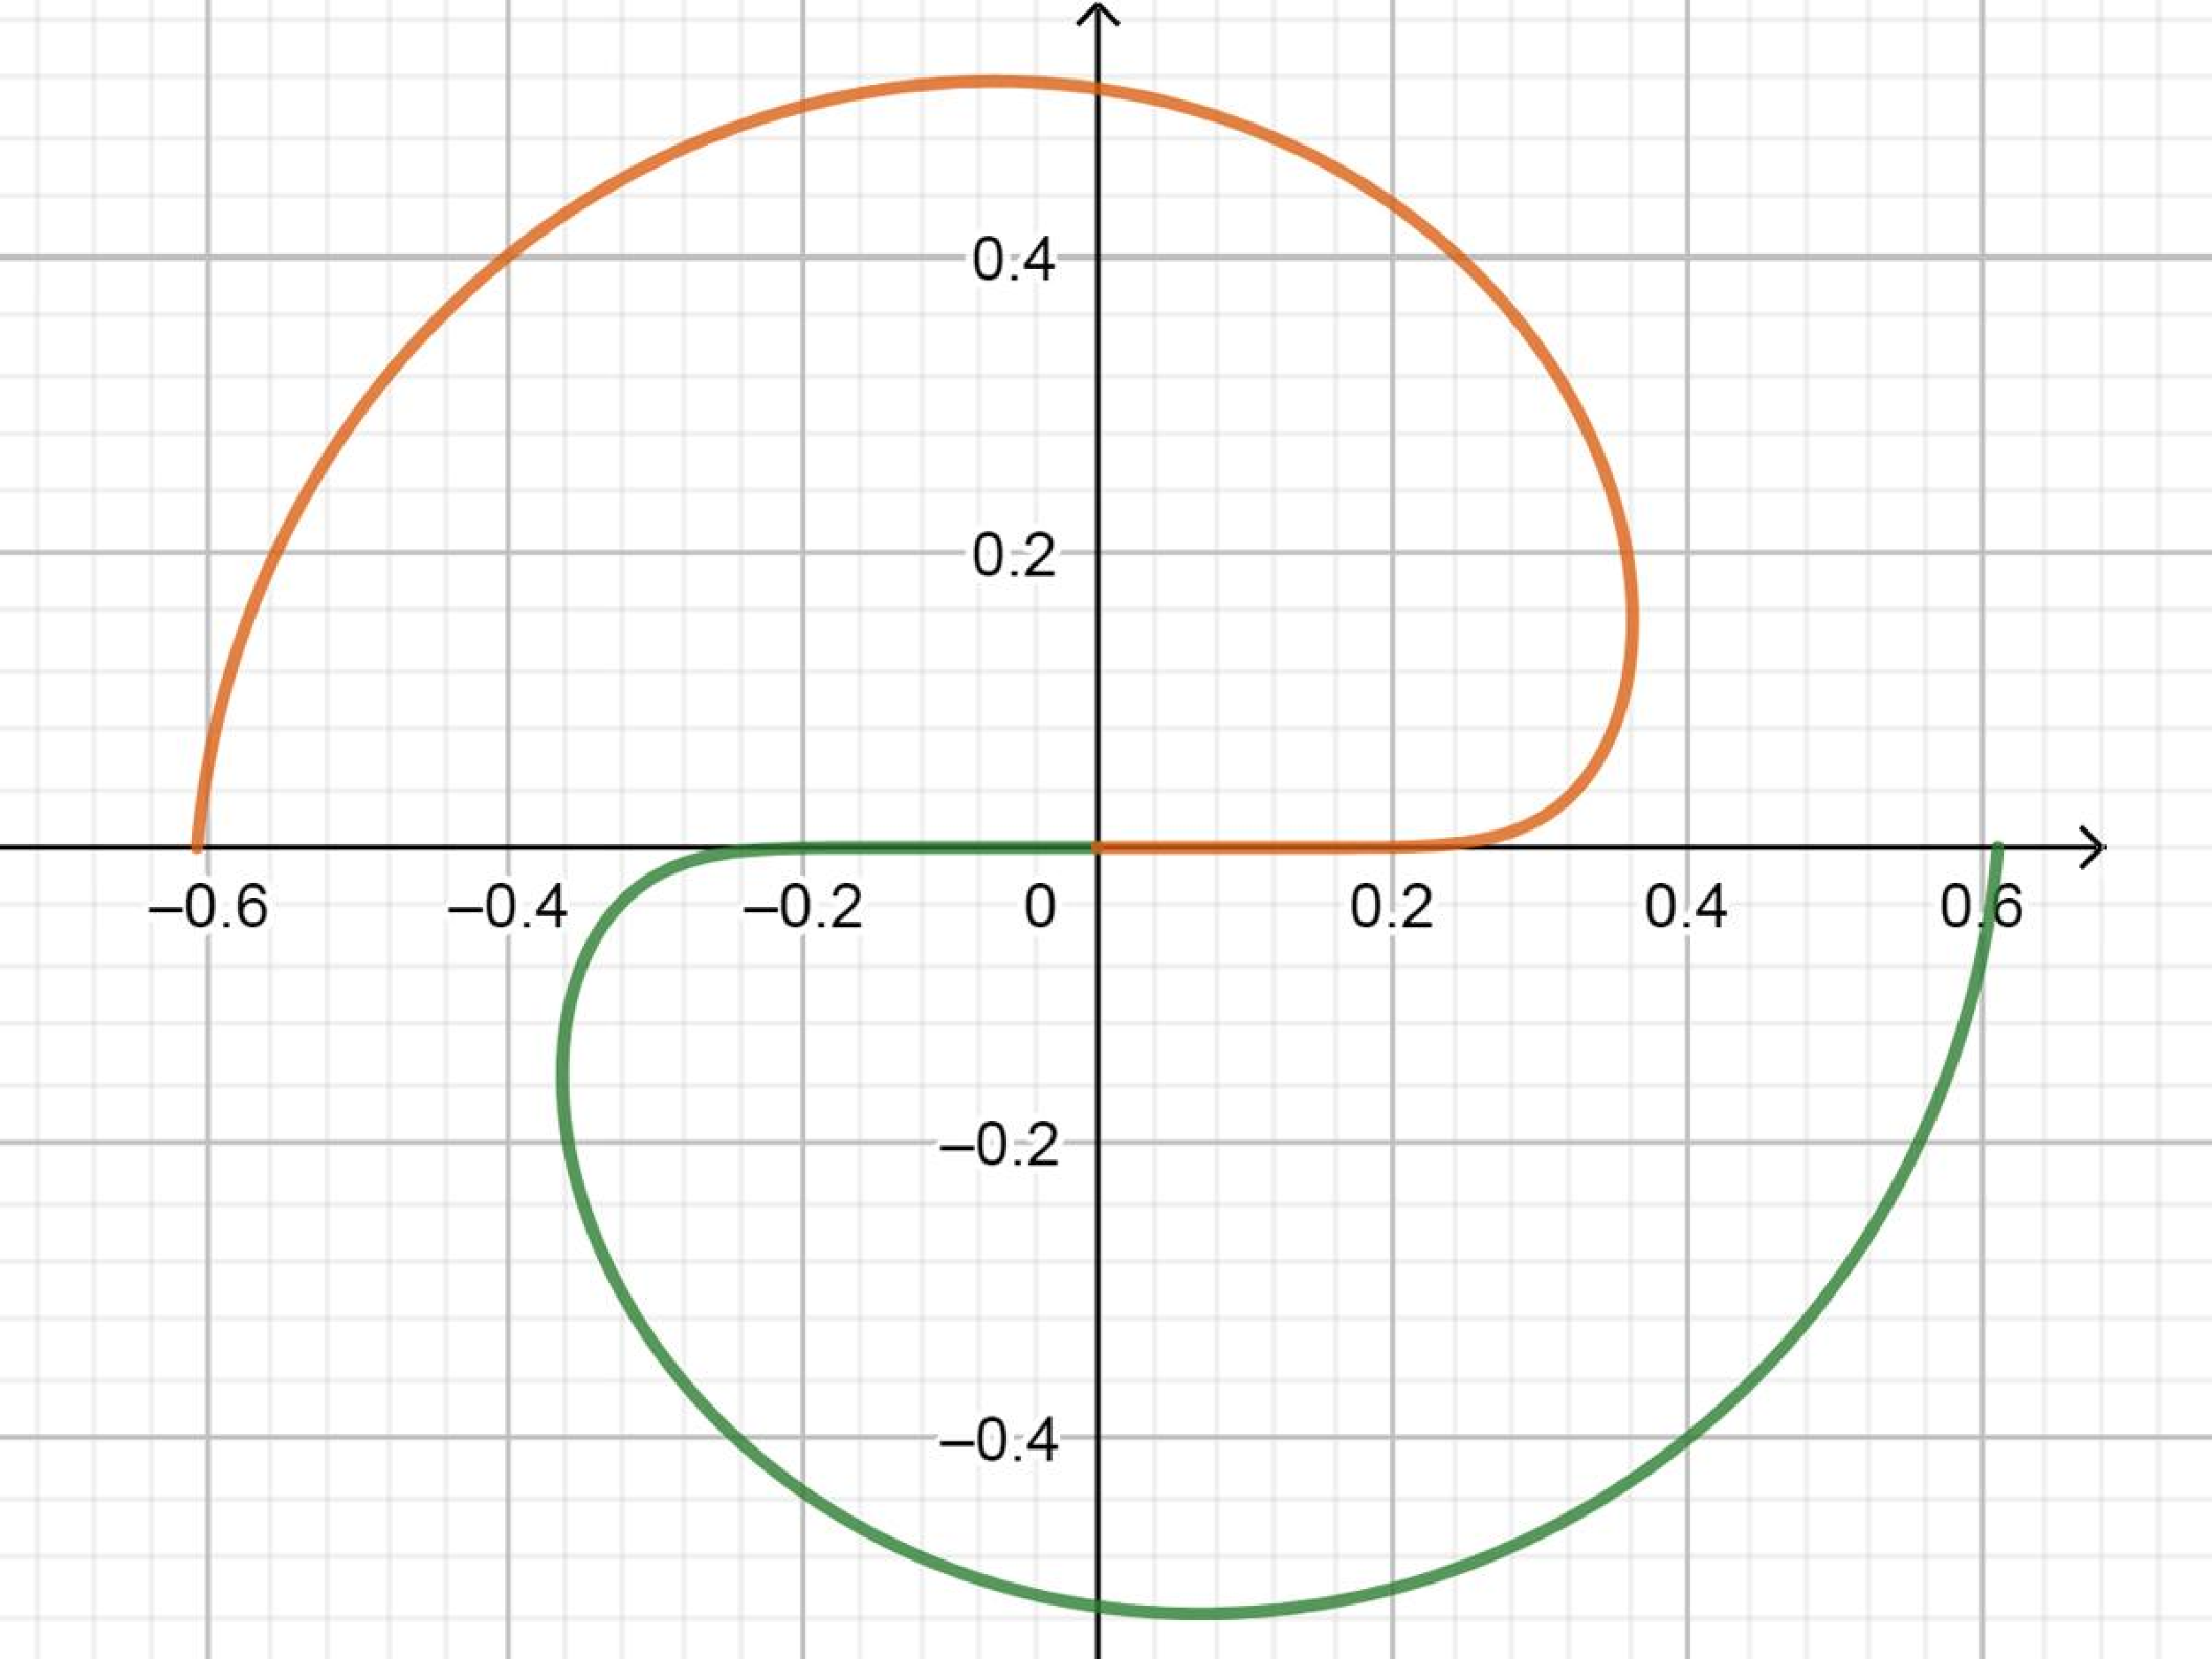
\includegraphics[width=0.2\textwidth]{ex1}}
	\subfigure[$B = 0.05, N = 2$]
		{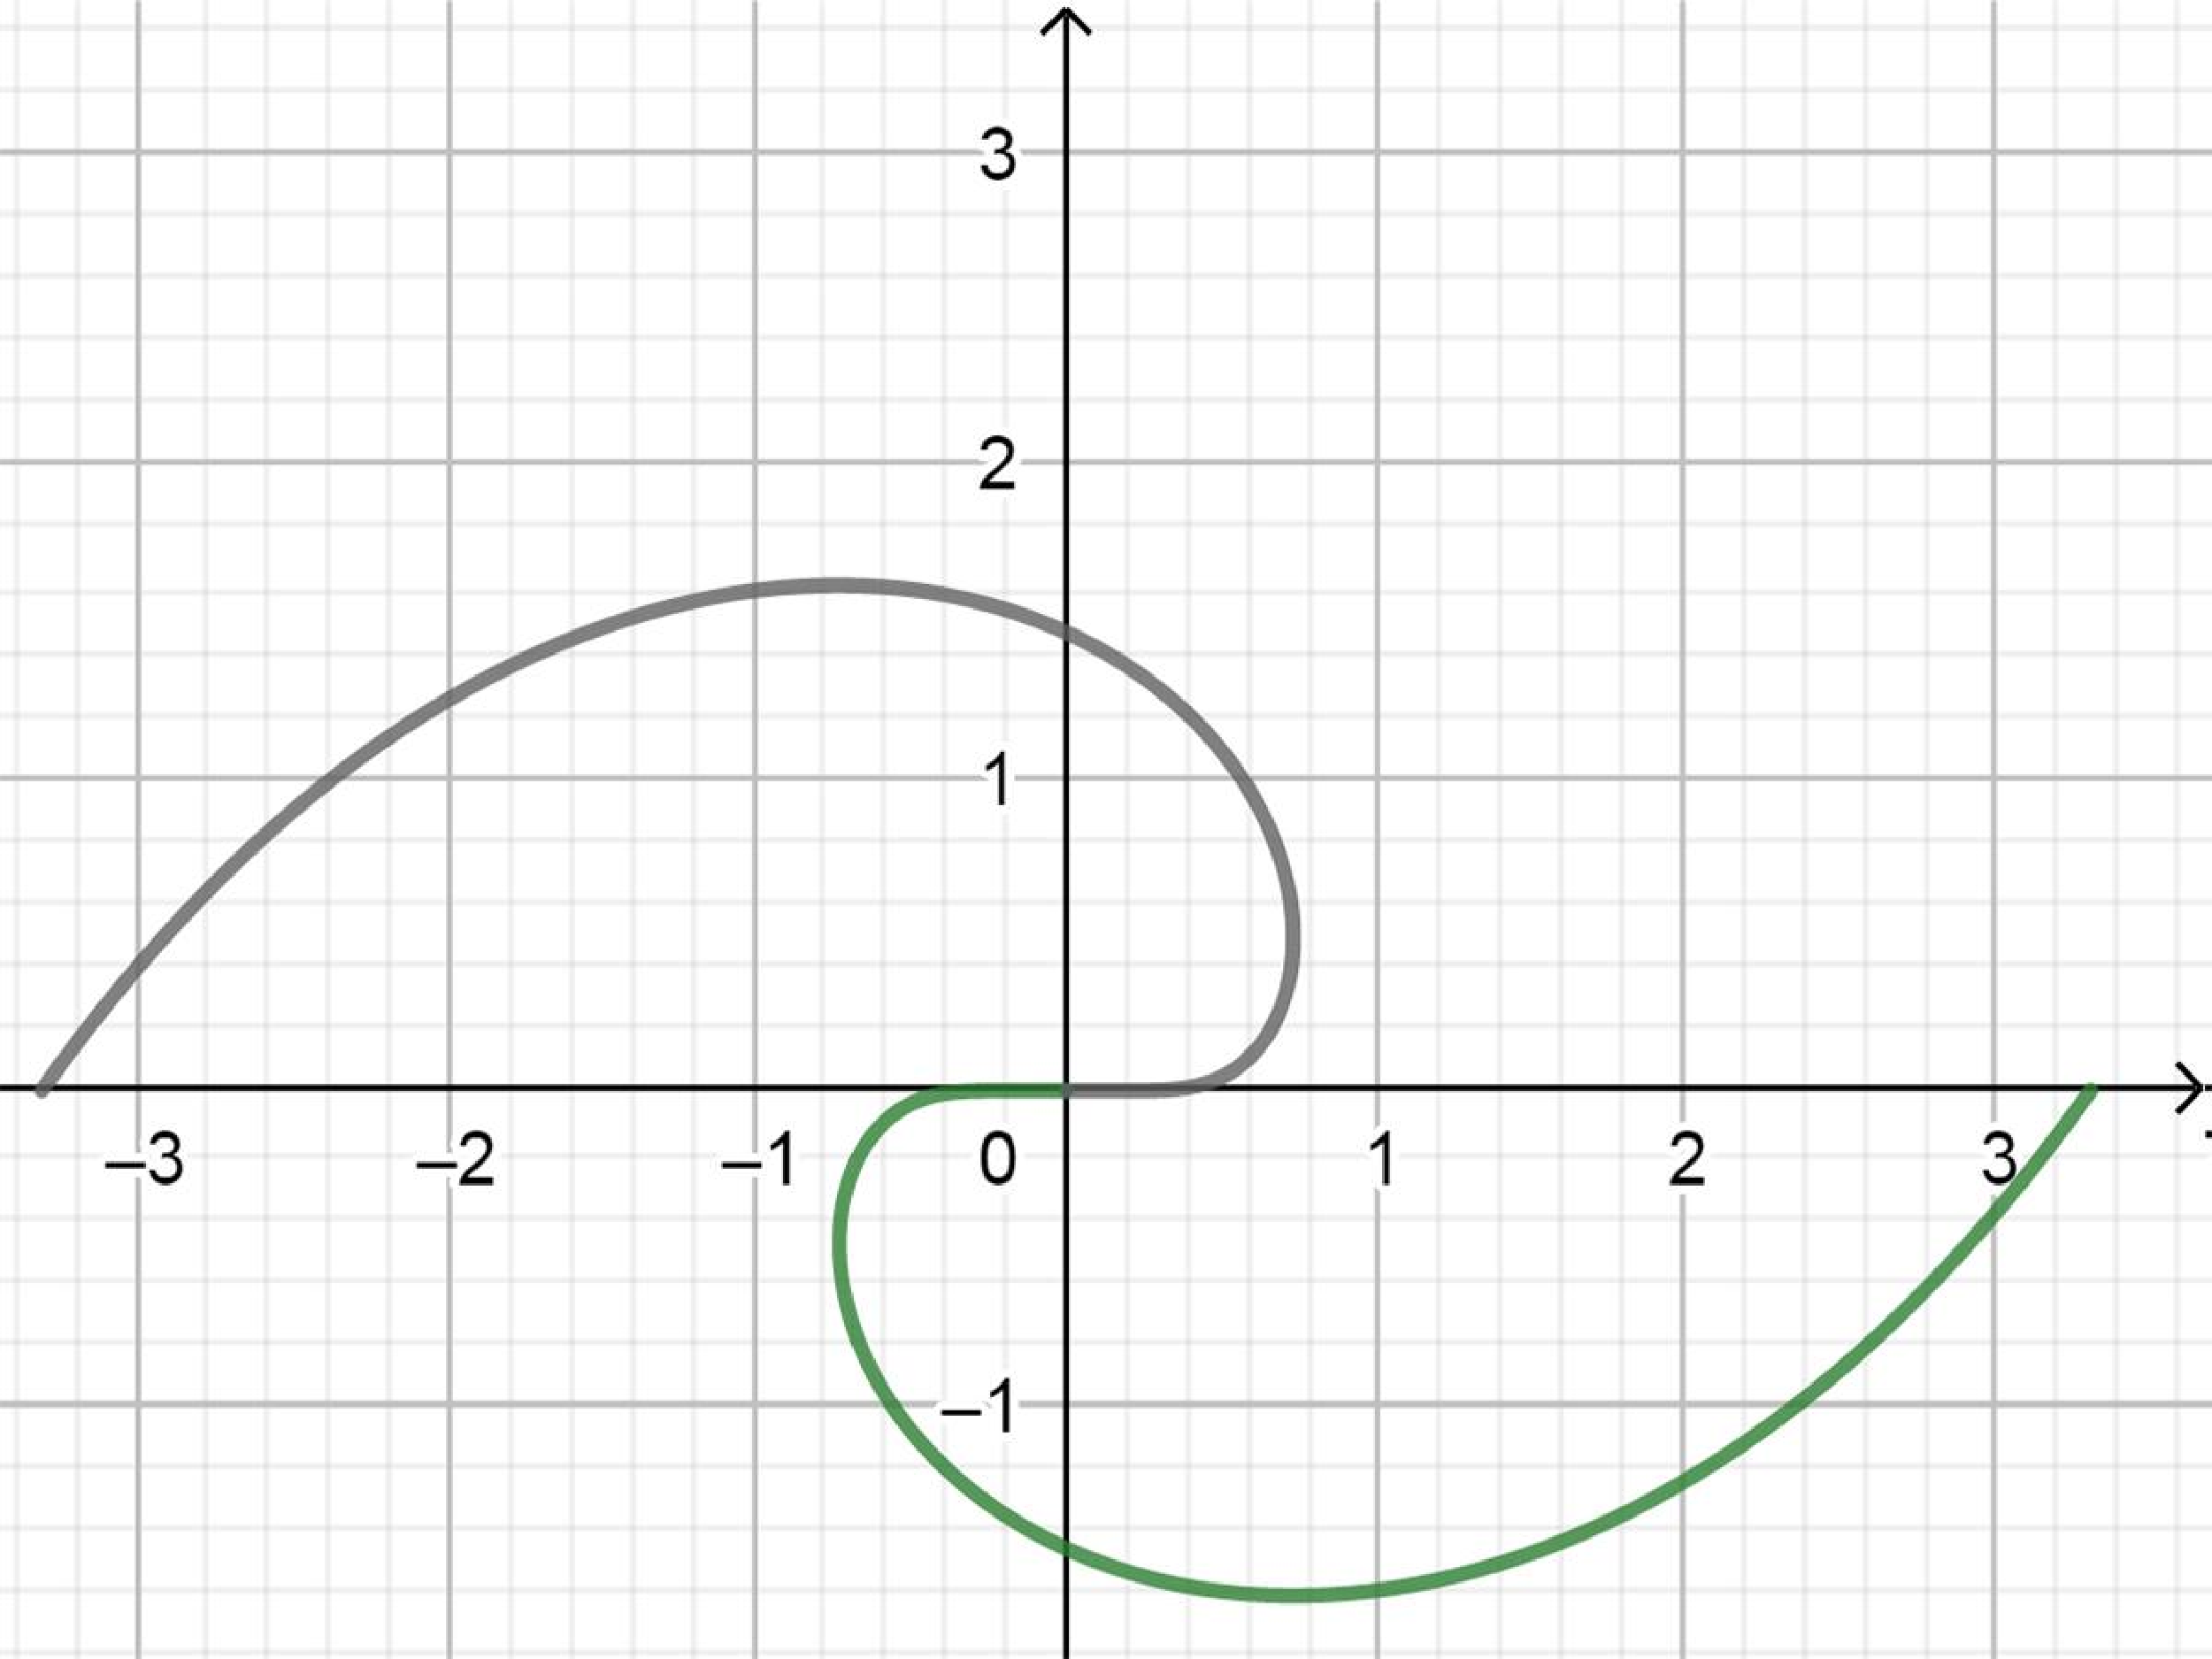
\includegraphics[width=0.2\textwidth]{ex2}}
\end{figure*}

\begin{figure*}[!h]
	\centering
	\subfigure[$B = 1.2, N = 2.1$]
		{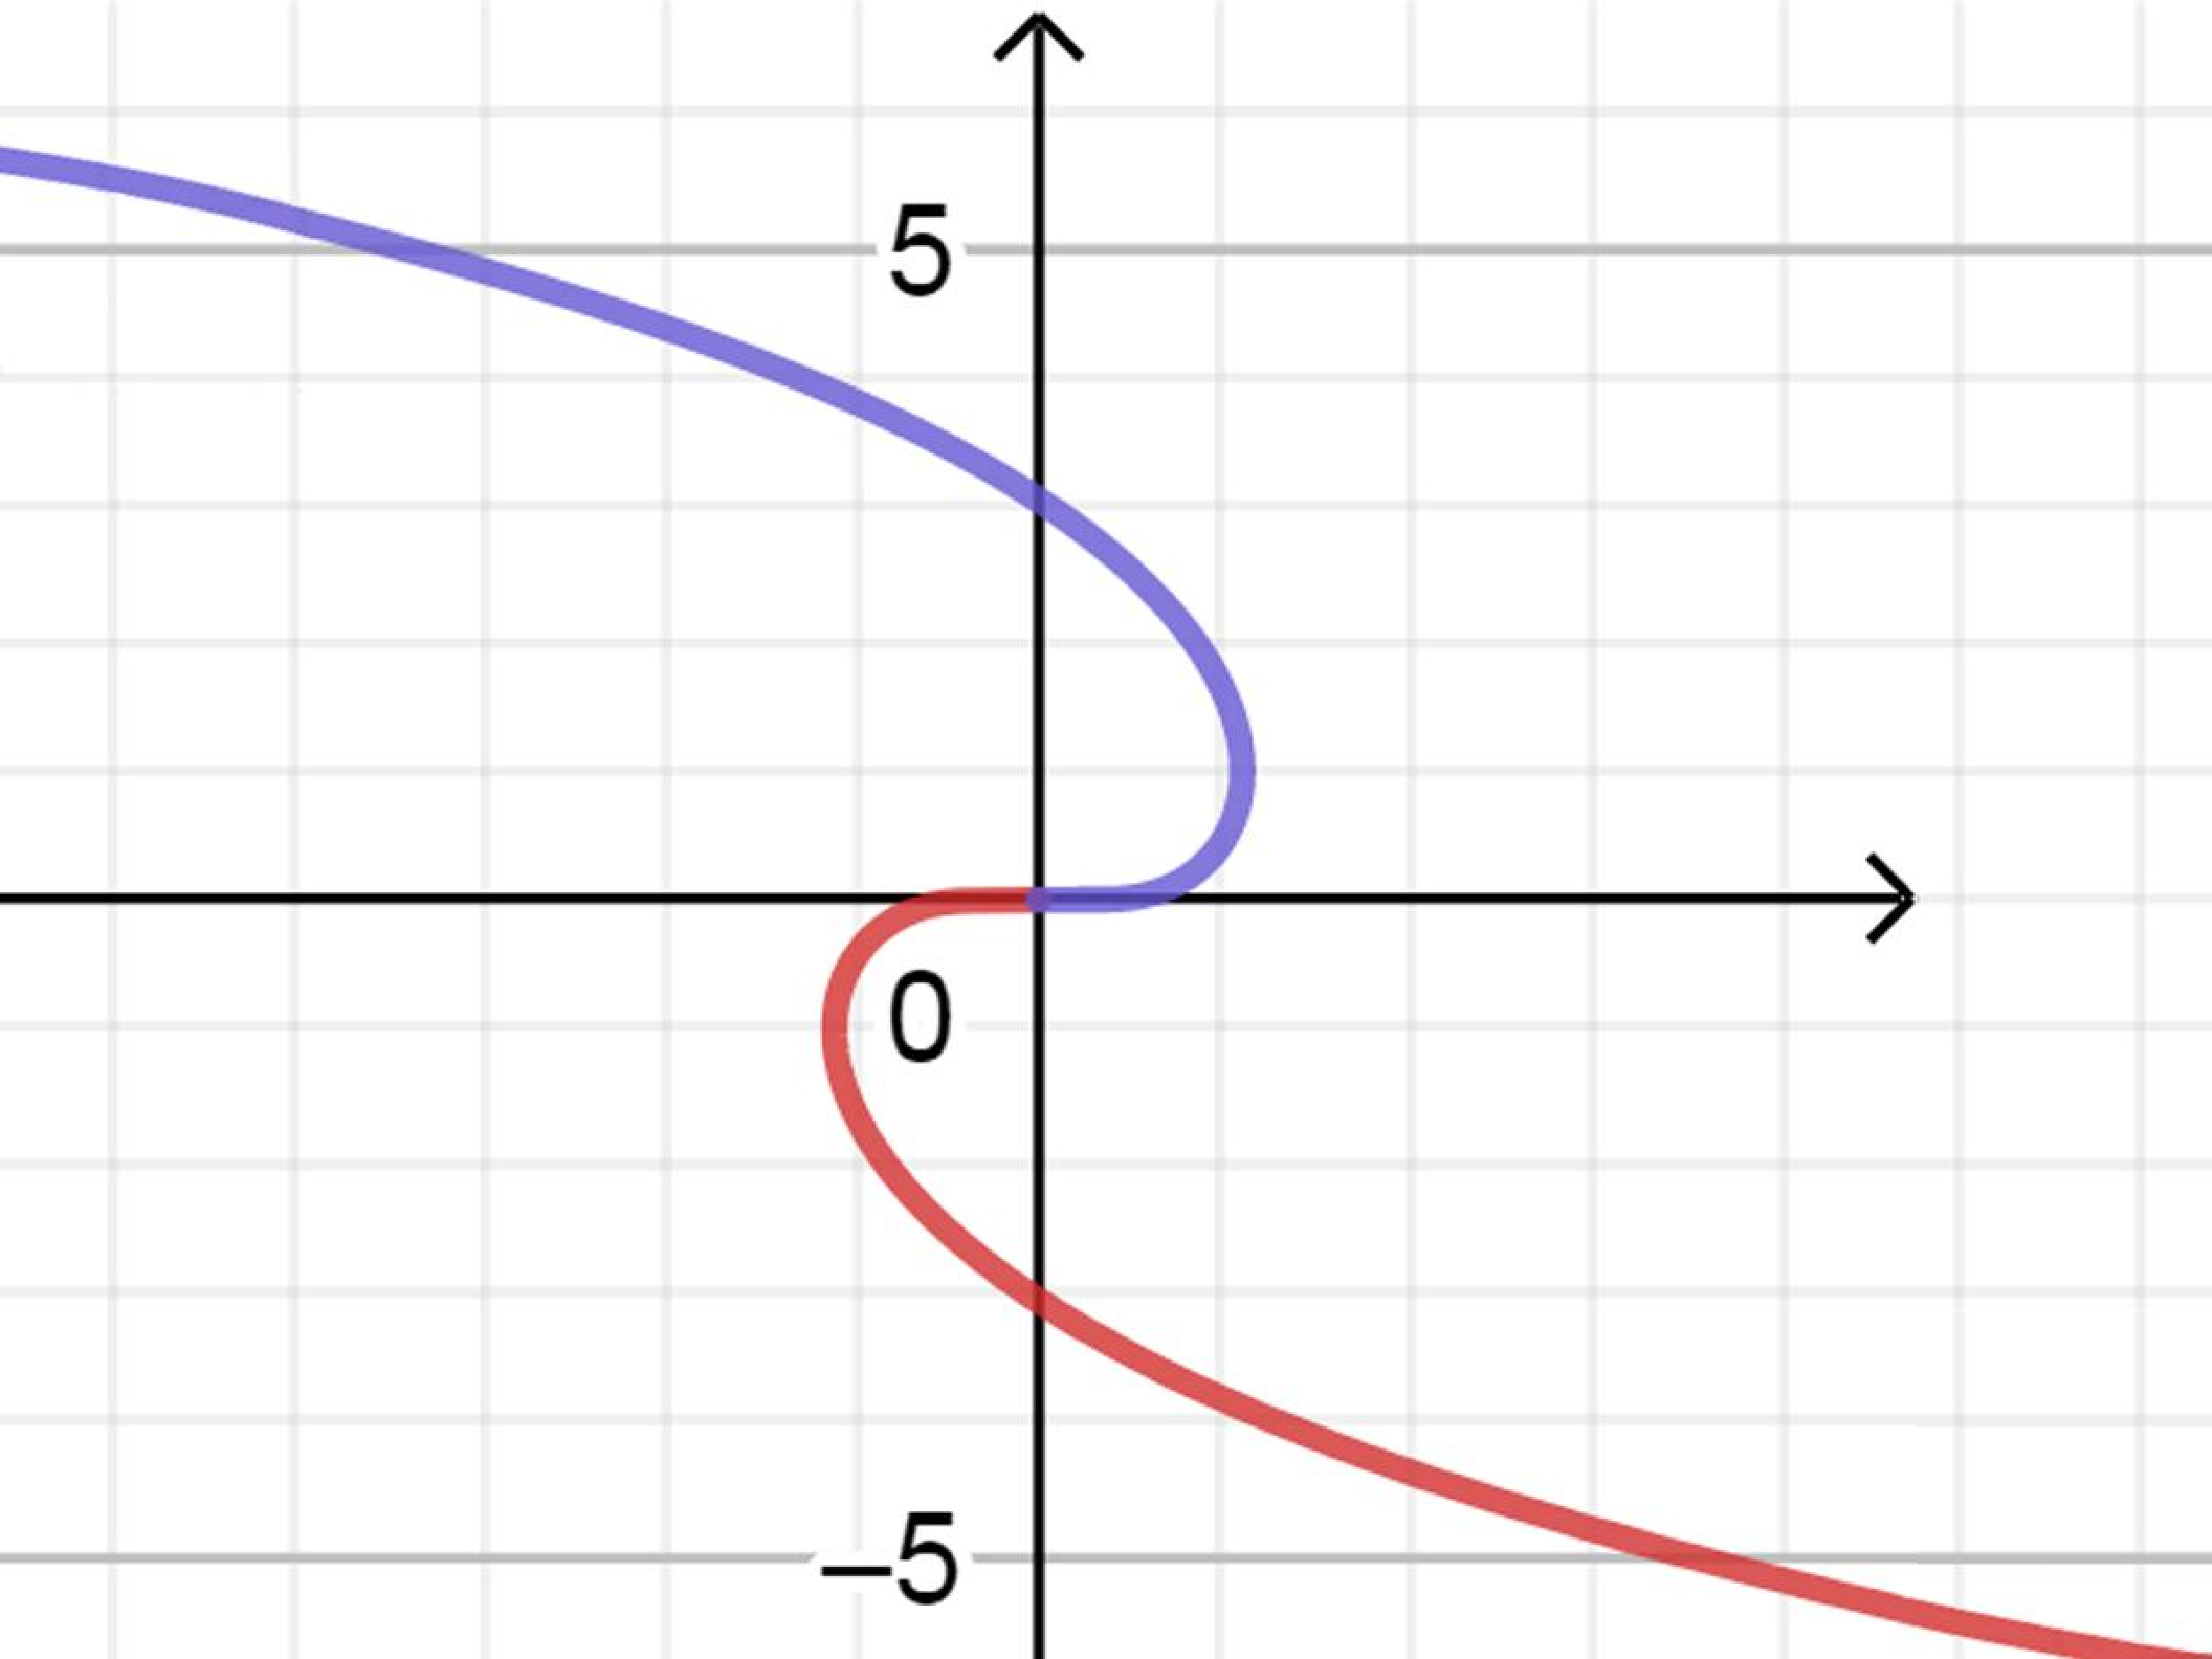
\includegraphics[width=0.2\textwidth]{ex3}}
	\subfigure[$B = 0.6, N = 4$]
		{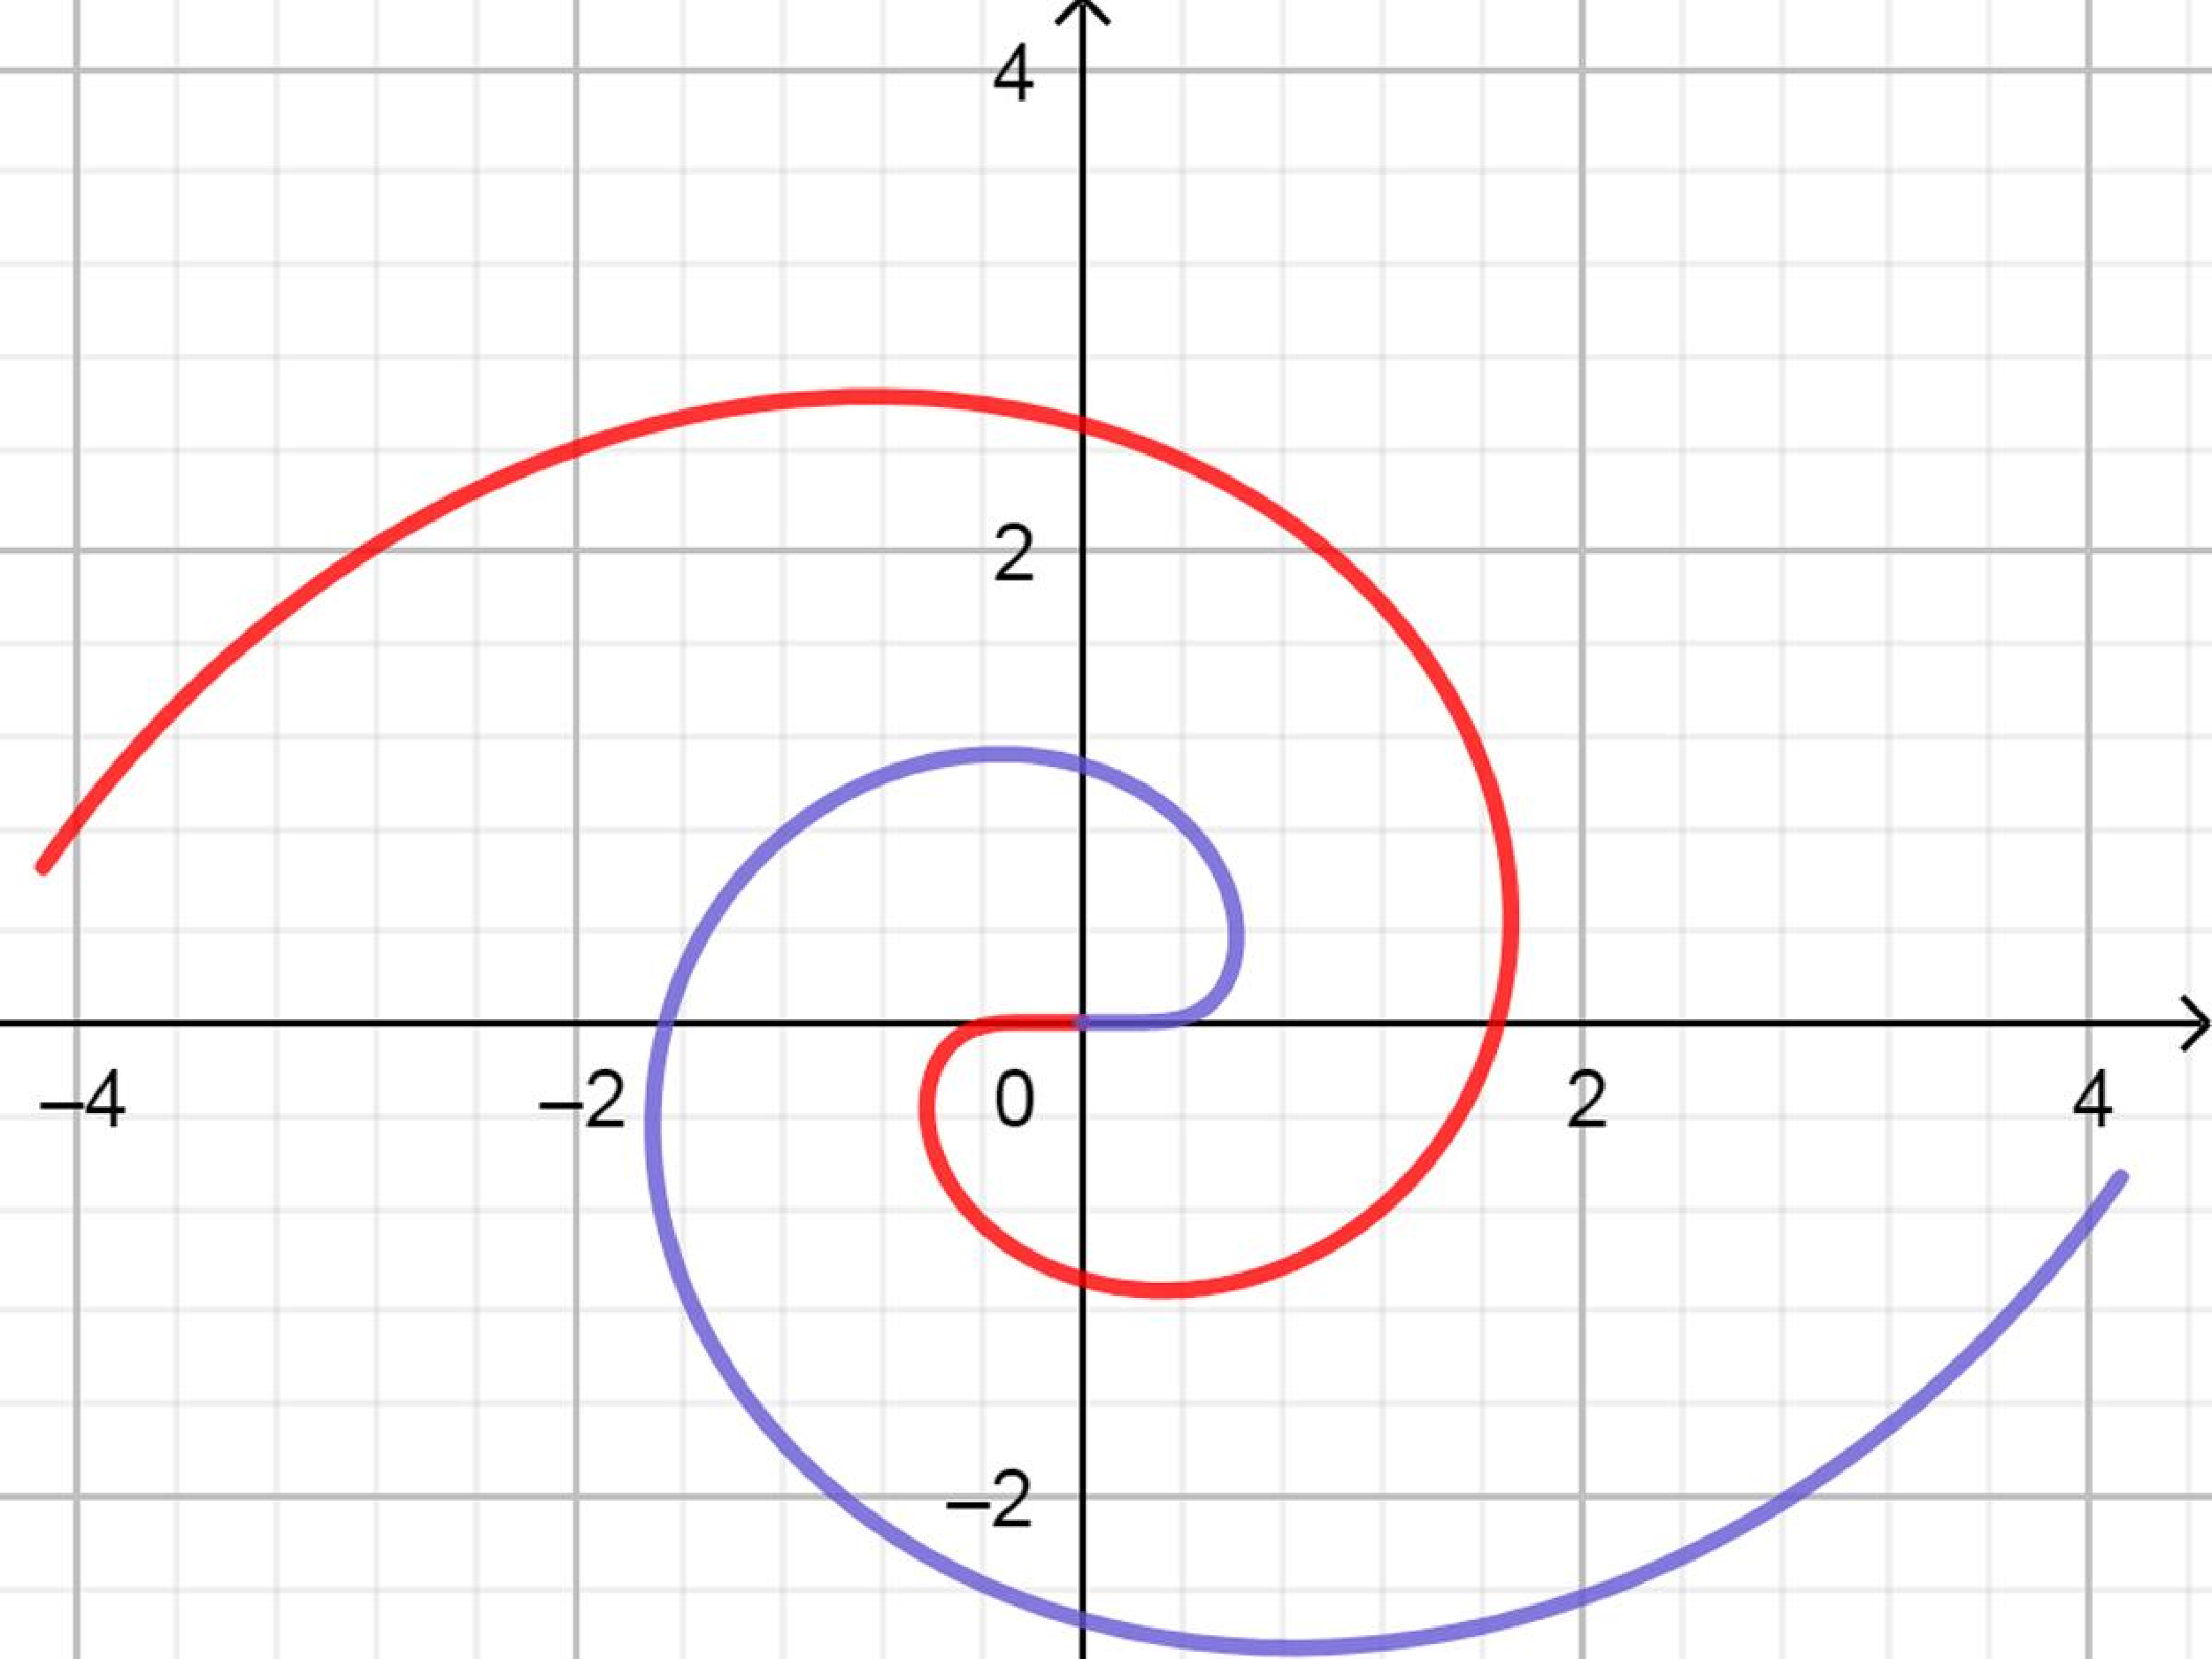
\includegraphics[width=0.2\textwidth]{ex4}}
	\caption{Exemplos de traços da equação \eqref{eq2}, para $N$ e $B$ variando.}
\end{figure*}

Nos exemplos dados é possível visualizar que pode-se formar adequadamente os membros das galáxias, observe que em cada figura foi usado uma função $f(x)$ e uma $-f(x)$ para podermos estruturar os "braços" do que seriam galáxias meramente ilustrativas, logo para encaixar os membros traçados, vale usar qualquer ferramenta do cálculo e obter os resultados necessários na formação das figuras, desde que a imagem da galáxia esteja fixada na origem do sistema de coordenadas. Veremos um exemplo plotando alguns traços de espirais sobre a imagem da galáxia NGC 1566 fotografada pelo telescópio Hubble WFC3 (ver figura 11).

\begin{figure}[!h]
	\centering
	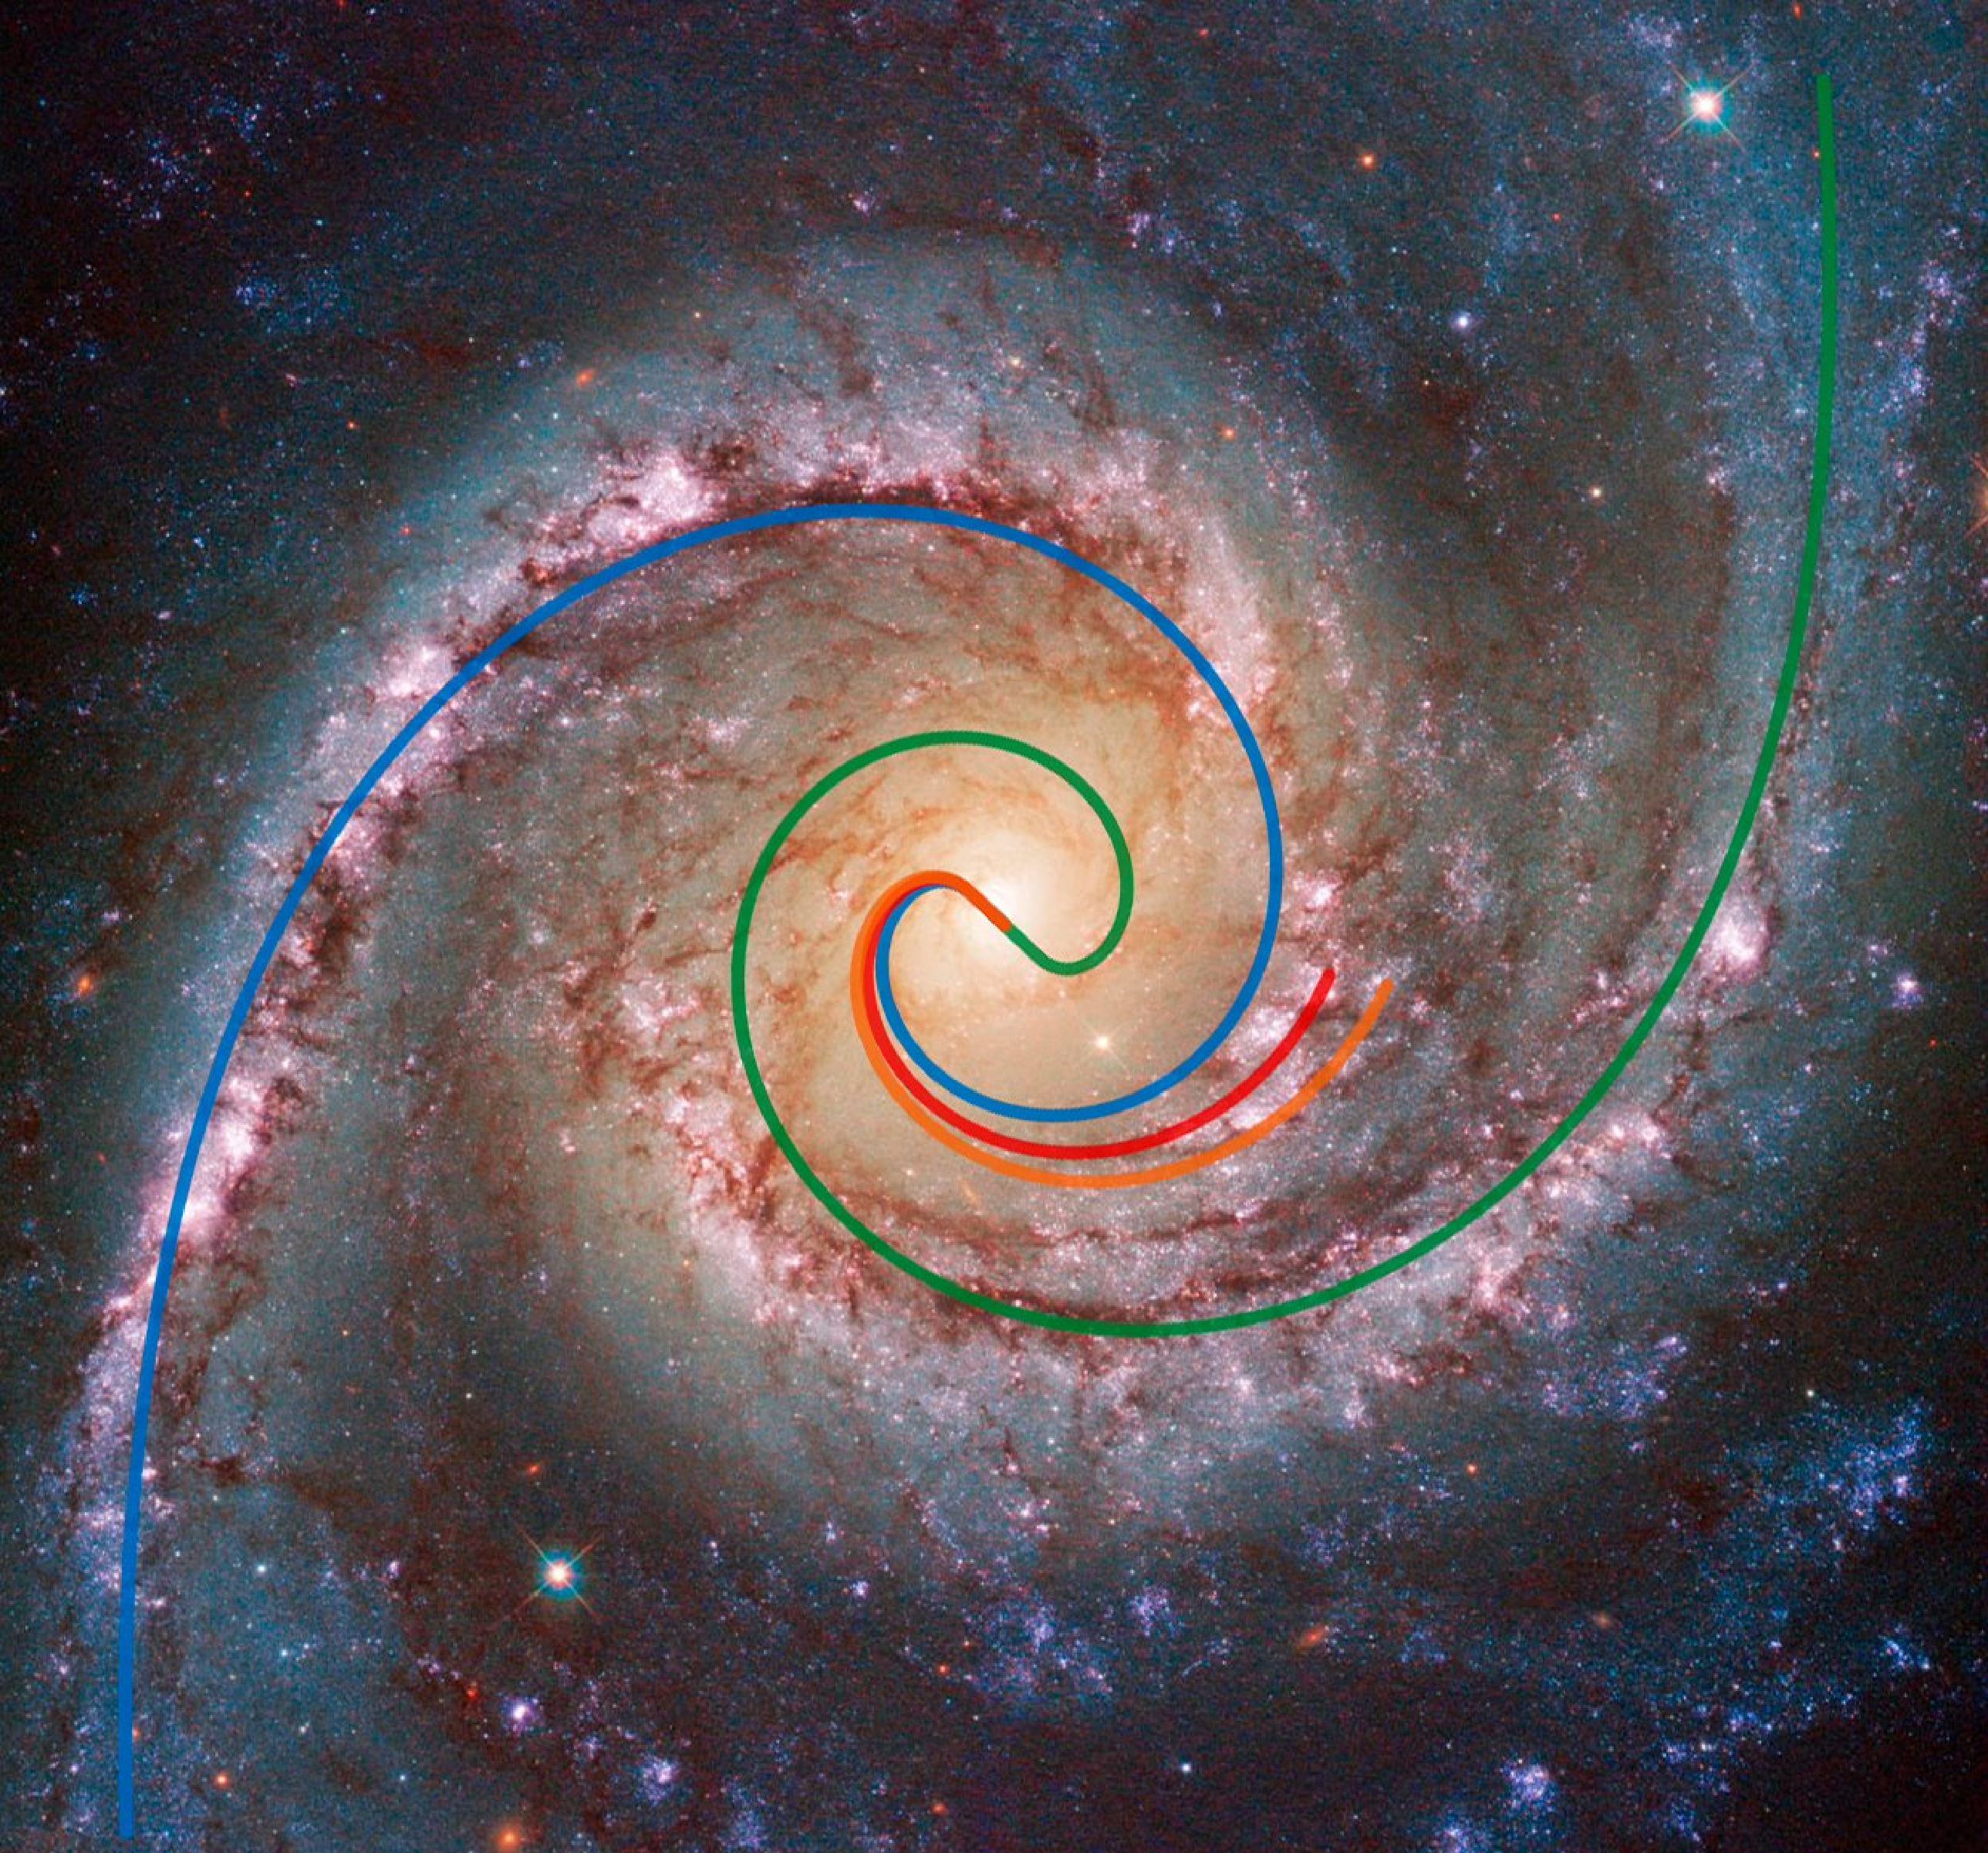
\includegraphics[width=0.3\textwidth]{NGC1566}
	\caption{Espirais geradas pela equação \eqref{eq2} cobrindo os membros da galáxia NGC 1566.}
\end{figure}

Na figura 11 foram plotadas quatro funções, parametrizadas como espirais a partir de \eqref{eq2}, para melhor entendermos como os elementos no espaço se comportam mediante a atração gravitacional, em direção ao centro da galáxias, escolhi uma das quatro funções, que na imagem aparece em azul, e chamei de $f$ descrita por $f(x) = \frac{1}{log\left(0.51\,tan\left(\frac{x}{8}\right)\right)}$.\\ \\ De $f$ foi feita uma outra parametrização com duas variáveis nos intervalos $[0, 2.5\pi]$ para $u$ e $[0 , \pi]$ para $z$, que dará origem a uma superfície plana, onde qualquer ponto contido nesse espaço gerado a partir da rotação de $f$ terá uma trajetória espiral, logo a terceira coordenada dessa transformação será $0$, pois se não produziria uma superfície não-plana. Esta transformação é oriunda da multiplicação do vetor que já tinha sido formado com a primeira parametrização $\left(\alpha(t) = (f(t)cos(t), f(t)sen(t))\right)$ e uma matriz de rotação, essa parametrização é caracterizada por:

\begin{equation*}
	\beta: \R^{2} \rightarrow \R^{3}
\end{equation*}

\begin{equation}\label{eq3}
	\alpha(u,z) = (f(u)cos(u)cos(z)+f(u)sen(u)sen(z), -f(u)cos(u)sen(z)+f(u)sen(u)cos(z)), 0).\,\, u, z \in \R
\end{equation}

\begin{figure}[!h]
	\centering
	\subfigure[Espaço gerado de $f$.]	
		{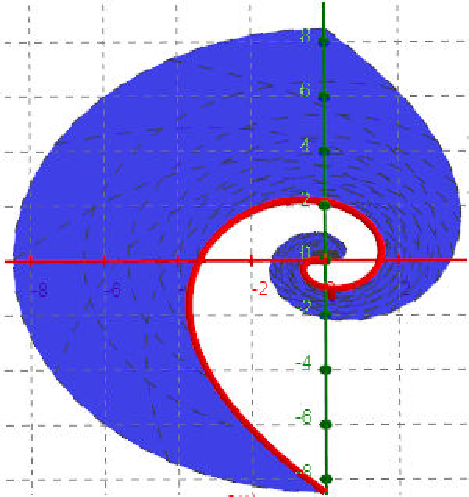
\includegraphics[width=0.3\textwidth]{es}}
	\subfigure[Pontos animados nas superfícies geradas pelas duas principais curvas da figura 11.]
		{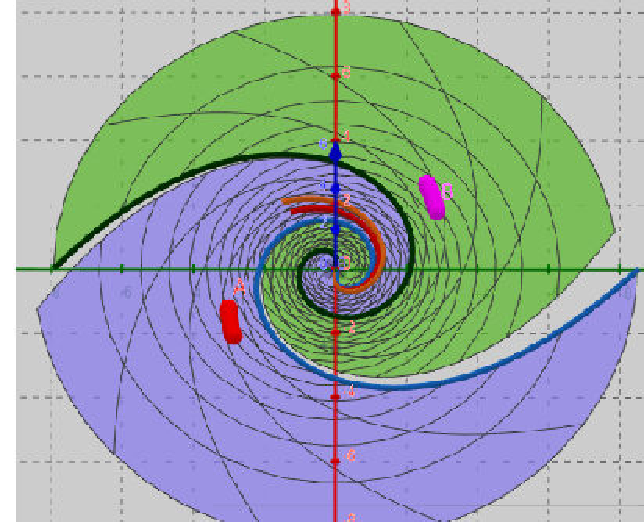
\includegraphics[width=0.35\textwidth]{p3}}
\end{figure}

\section{Construção utilizando Geogebra}
	Com base na definição de espiral arquimediana, onde um ponto se move numa variação constante ao longo da linha reta, começando pela extremidade que permanece fixa, extremidade chamada de origem, utilizaremos o software Geogebra, em sua versão online, e suas ferramentas de construção, para então a partir de uma animação visualizar como se forma uma espiral arquimediana e suas particularidades.
\clearpage
\begin{enumerate}
	\item Criemos uma circunferência de raio $n$
		\begin{figure}[!h]
			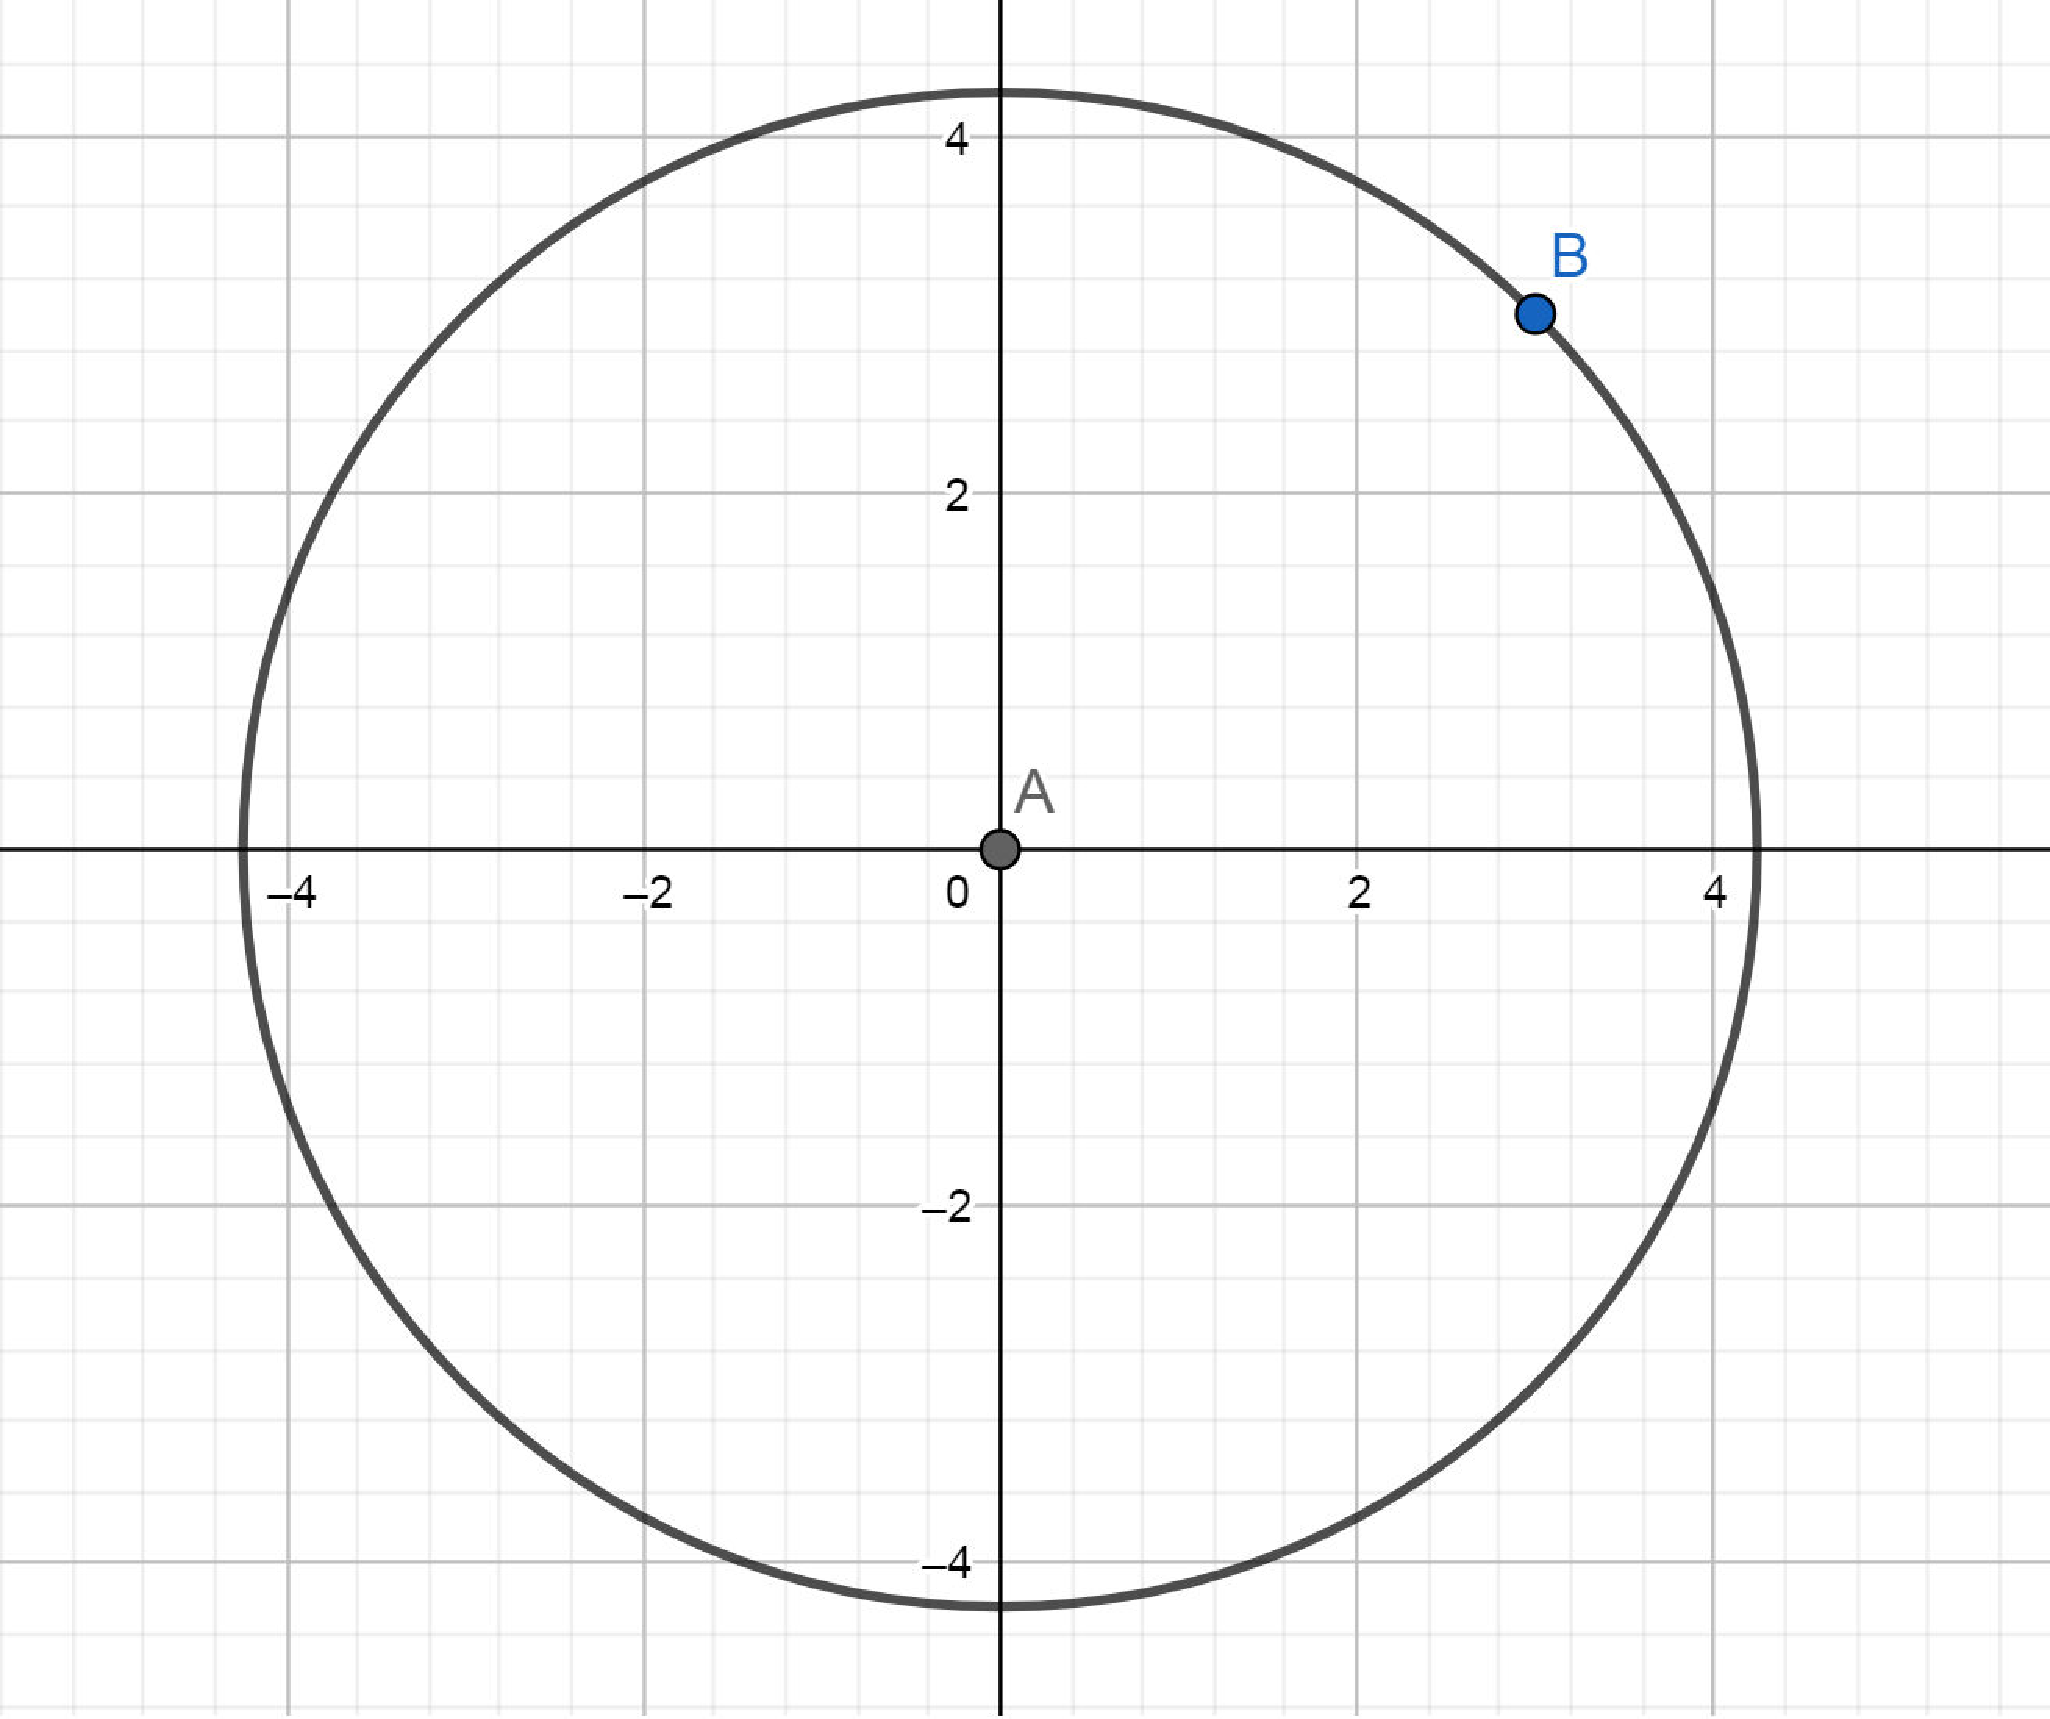
\includegraphics[width=0.3\textwidth]{c1}
		\end{figure}
	\item Agora com ligamos um segmento de reta $CD$ do centro até um ponto qualquer do traço da circunferência, utilizando sempre o botão direito do mouse para acessar as opções relacionadas aos objetos, então fixamos o ponto $C$
		\begin{figure}[!h]
			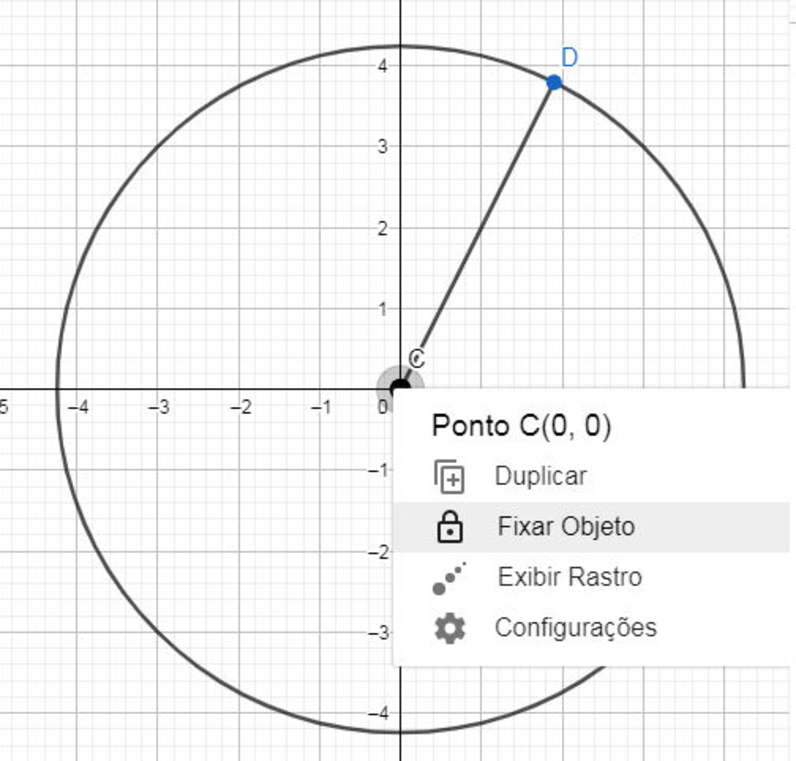
\includegraphics[width=0.3\textwidth]{c2}
		\end{figure}
	\item Plotando um ponto qualquer sobre o segmento de reta, usamos a ferrementa "Animação", tanto no ponto $E$ quanto no $D$, e em seguida façamos com que nos mostre o rastro gerado por $E$, enquanto animado.
		\begin{figure}[!h]
			{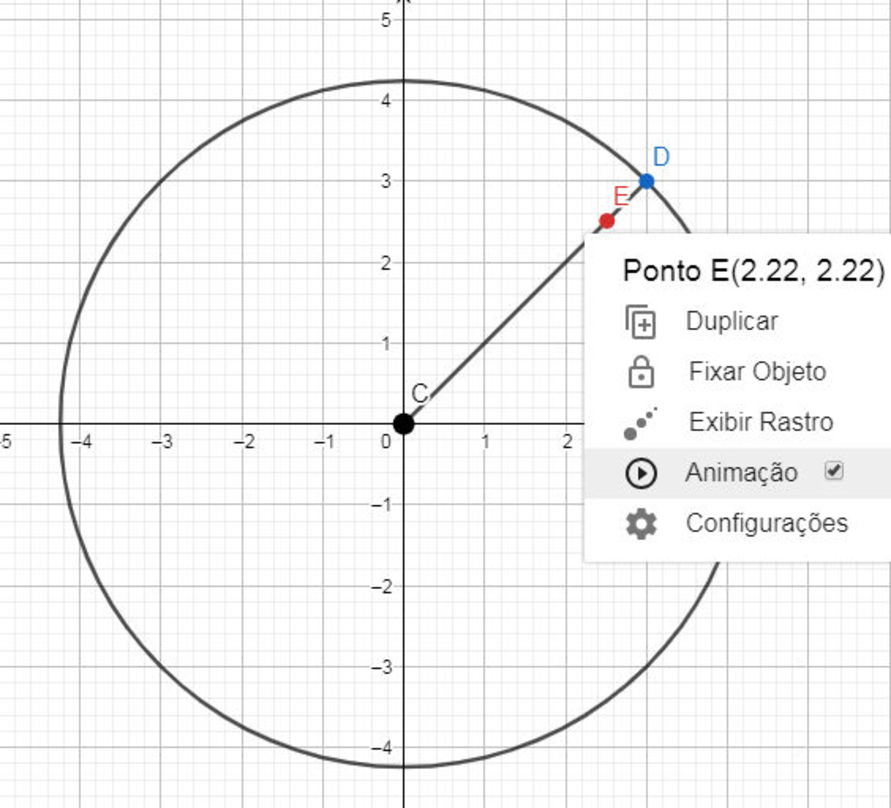
\includegraphics[width=0.4\textwidth]{c3}}
			{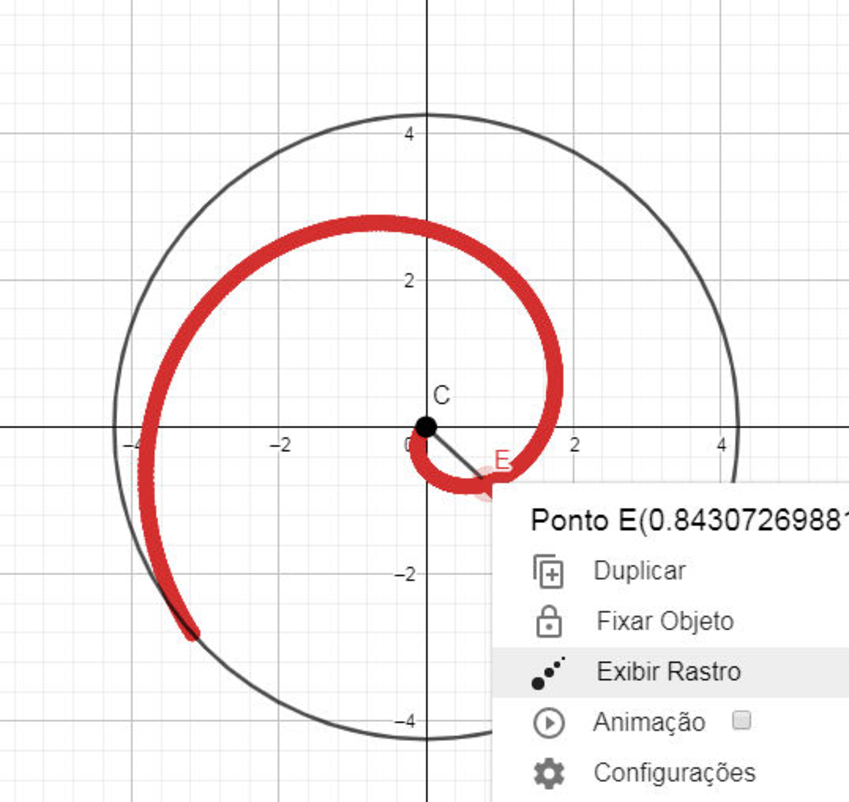
\includegraphics[width=0.4\textwidth]{c4}}
		\end{figure}
\end{enumerate}

Logo a partir dessa animação, e as ferramentas dispostas pelo software, podemos fazer diversas observações, explorando por exemplo, a velocidade com qual o ponto $E$ se move no segmento, ou a velocidade do ponto $D$, que por consequência, varia a velocidade de rotação do segmento. (Ver figuras 13 e 14).
\clearpage

\begin{figure}[!h]
	{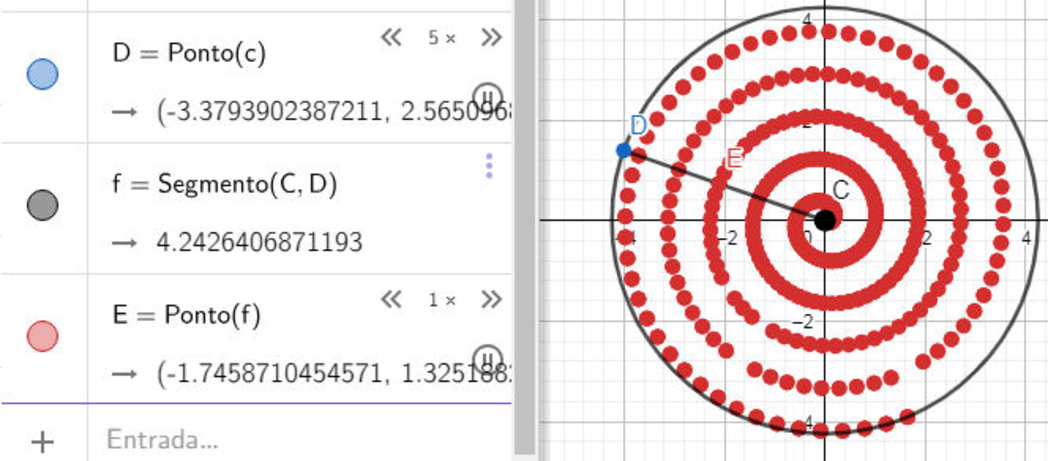
\includegraphics[width=0.4\textwidth]{c5}}
		\caption{Traço da espiral com $D$ movendo-se $5$x mais rápido.}
	{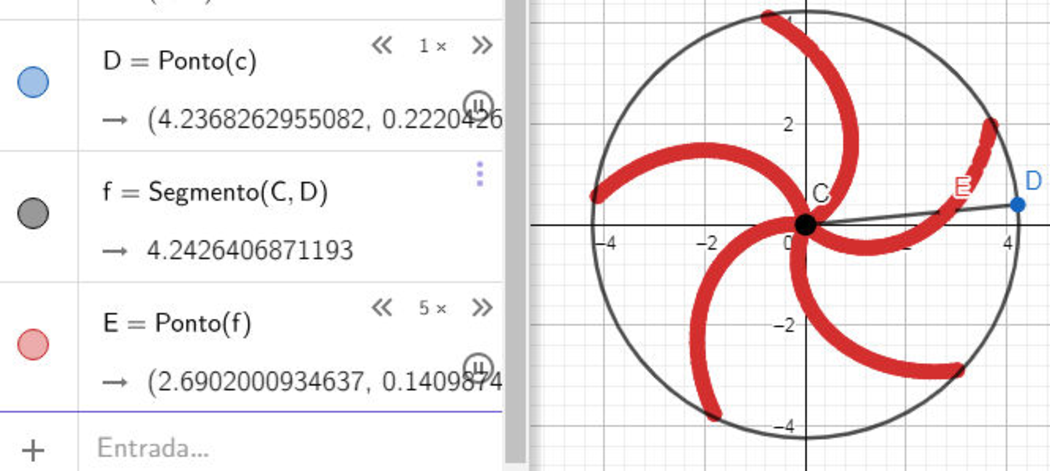
\includegraphics[width=0.4\textwidth]{c6}}
		\caption{Traço da espiral com $E$ movendo-se $5$x mais rápido.}
\end{figure}

\section{Relato de Experiência}
Apresentamos aqui um breve relado sobre um minicurso de Parametrizações usando o Geogebra e o laboratório de computação científica do Instituto de Física e Matemática, logo destinado a estudantes dos cursos de Física e Matemática da UFPEL, o cronograma ficou dividido em três encontros e duração de 3h. No primeiro dia, foi discutido sobre o que seria uma espiral, e então a apresentamos da definição de espiral de Arquimedes, a partir da compreensão desses dois quesitos. Foi apresentado o passo a passo da construção da espiral arquimediana, no Geogebra, que então foi reproduzida e explorada pelos ouvintes. Logo falamos sobre os principais tipos de espirais, já conhecidas e estudadas.\\
No Segundo dia de minicurso, foi ministrada uma palestra sobre galáxias, pela professora de Astronomia Virgínia Mello, introduzindo os tipos de galáxias, e como cada uma é formada, e as diferentes particularidades dessas formações, e a formação das infinitas estrelas e aglomerados estelares se unirem formando um grande sistema, gravitacionalmente ligado.\\
No terceiro dia, foi trado sobre parametrizações de espirais, e por fim apresentei a equação de parametrização \eqref{eq2}, para que a partir dela explorassem a parametrização dos membros de uma galáxia, oriundas de imagens por eles escolhidas como as figuras abaixo, com as parametrizações feitas pelo ouvinte.

\begin{figure}[!h]
	{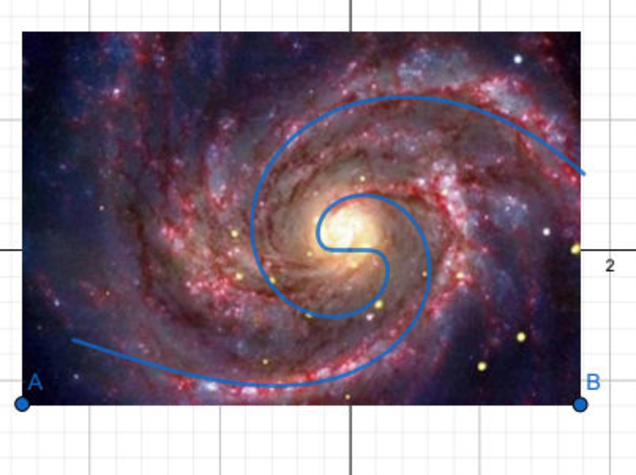
\includegraphics[width=0.4\textwidth]{t1}}
	{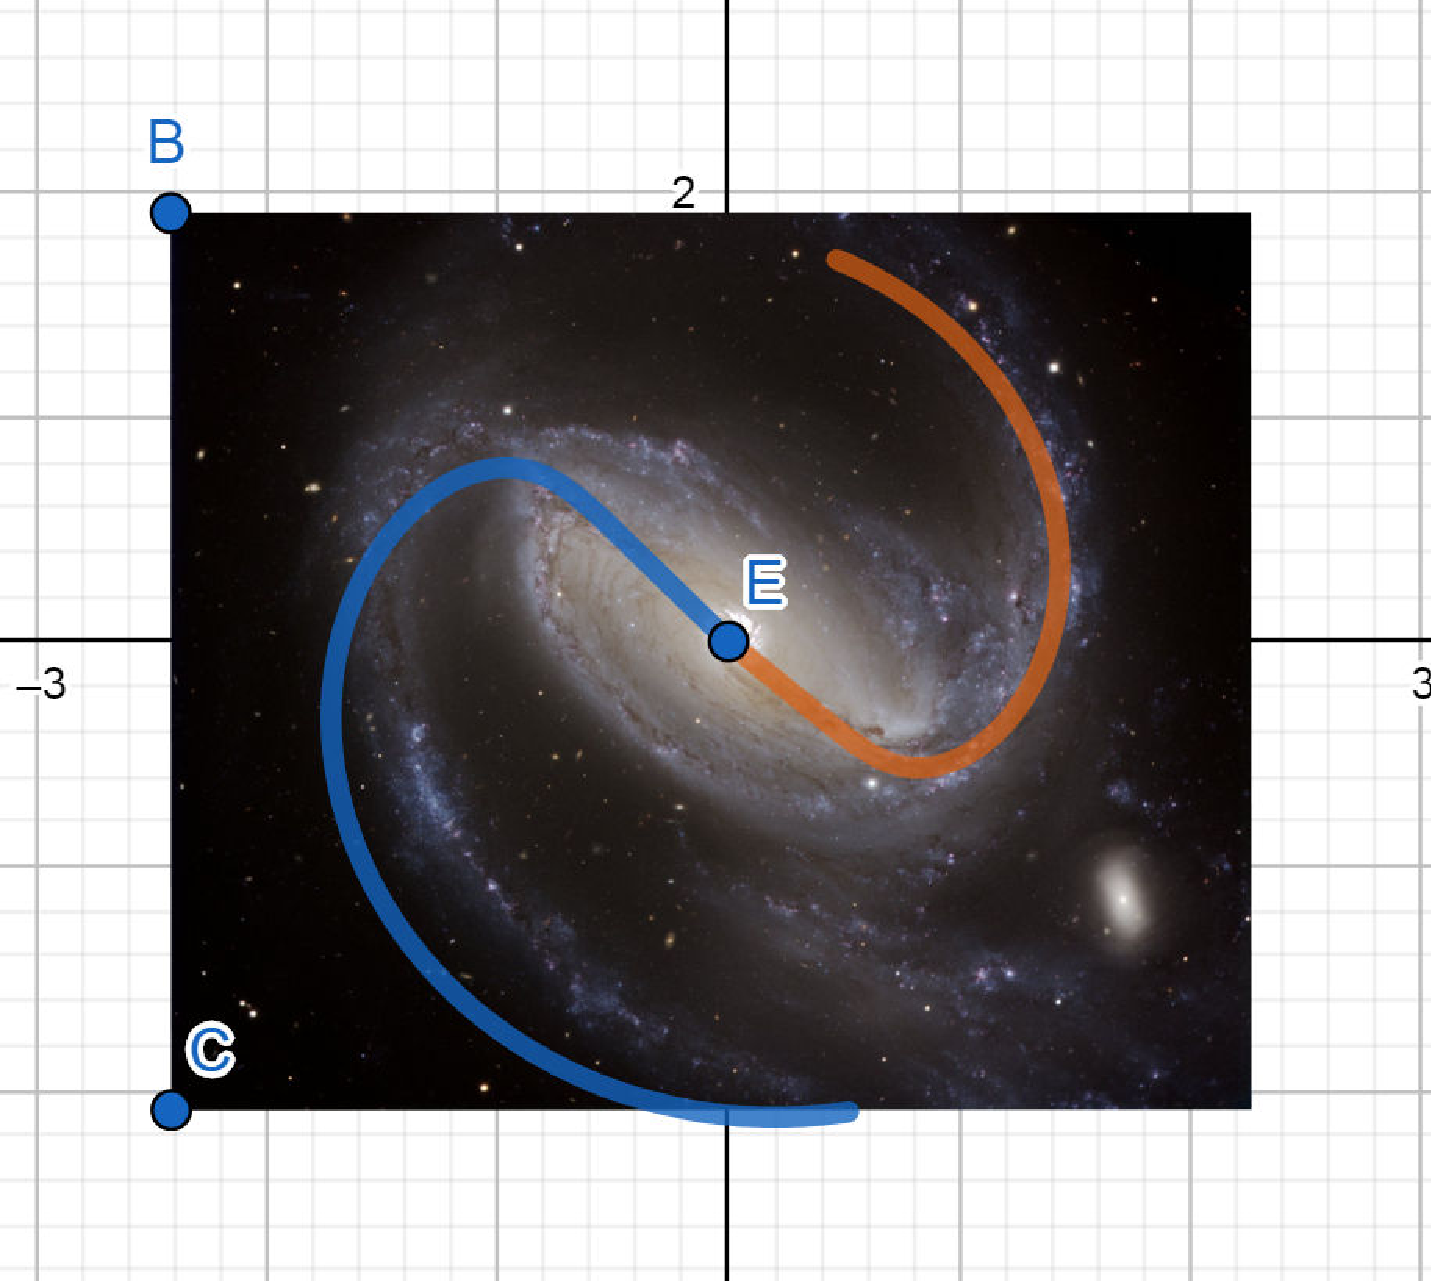
\includegraphics[width=0.4\textwidth]{t2}}
\end{figure}
\clearpage

\section{Conclusões}

O principal resultado obtido neste trabalho foi a parametrização \eqref{eq3}, em que nos permite criar uma superfície na qual podemos relacionar a trajetória de um ponto com as curvas da superfície plana, concluindo que através da \eqref{eq2} podemos simular esta trajetória ligada a superfície. Logo a partir da definição de Arquimedes, onde temos que um ponto se afasta ou se aproxima da origem, os traços são formados a partir da aproximação dos pontos pertencentes ao raio em direção a origem. Assim obtemos uma noção da trajetória dos corpos de uma galáxia.\\
Ao abordar o que é uma parametrização buscamos oferecer uma ferramenta que nos possibilita modelar as estruturas de uma galáxia, fazer ciência diz respeito a exatamente isto, modelar a natureza a nossa volta, formalmente, e coerente com os fenômenos observados. Apresentar estes conceitos aos ouvintes do minicurso permitiu contribuir para a noção do uso das ferramentas do cálculo e da álgebra linear, de forma mais intuitiva, e com auxílio do Geogebra, podendo assim contemplar estudantes de qualquer semestre dos cursos de física ou matemática.%----------------------------------------------------------------------------------------
%	REFERENCE LIST
%----------------------------------------------------------------------------------------

% inclusão de referências utilizando BibTeX
\bibliographystyle{cen}
\bibliography{exemplo_bib_cen}


\end{document}
